\documentclass{vkr}
\usepackage[english, russian]{babel} % переносы
\usepackage{graphicx} % для вставки картинок
\graphicspath{{images/}} % путь к изображениям
\usepackage[hidelinks]{hyperref}
\usepackage{float} % определяет метод H для рисунка с переносом на следующую страницу, ели не помещается
\usepackage{pdflscape}
\addto{\captionsrussian}{\renewcommand{\refname}{СПИСОК ИСПОЛЬЗОВАННЫХ ИСТОЧНИКОВ}}
\usepackage{xltabular} % для вставки таблиц
\usepackage{makecell}
\renewcommand\theadfont{} % шрифт в /thead
\usepackage{array} % для определения новых типов столбцов таблиц
\newcolumntype{T}{>{\centering\arraybackslash}X} % новый тип столбца T - автоматическая ширина столбца с выравниванием по центру
\newcolumntype{R}{>{\raggedleft\arraybackslash}X} % новый тип столбца R - автоматическая ширина столбца с выравниванием по правому краю
\newcolumntype{C}[1]{>{\centering\let\newline\\\arraybackslash\hspace{0pt}}m{#1}} % новый тип столбца C - фиксированная ширина столбца с выравниванием по центру
\newcolumntype{r}[1]{>{\raggedleft\arraybackslash}p{#1}} % новый тип столбца r - фиксированная ширина столбца с выравниванием по правому краю
\newcommand{\centrow}{\centering\arraybackslash} % командой \centrow можно центрировать одну ячейку (заголовок) в столбце типа X или p, оставив в оcтальных ячейках другой тип выравнивания
\newcommand{\finishhead}{\endhead\hline\endlastfoot}
\newcommand{\continuecaption}[1]{\captionsetup{labelformat=empty} \caption[]{#1}\\ \hline }
\usepackage{etoolbox}
\AtBeginEnvironment{xltabular}{\refstepcounter{tablecnt}} % подсчет таблиц xltabular, обычные таблицы подсчитываются в классе

\usepackage[tableposition=top]{caption} % подпись таблицы вверху
\captionsetup{strut=off}
\setlength{\intextsep}{0pt} % Vertical space above & below [h] floats
\setlength{\textfloatsep}{0pt} % Vertical space below (above) [t] ([b]) floats
\DeclareCaptionLabelFormat{gostfigure}{Рисунок #2} %подпись рисунка
\DeclareCaptionLabelFormat{gosttable}{Таблица #2} %подпись таблицы
\DeclareCaptionLabelSeparator{gost}{~--~} %разделитель в рисунках и таблицах
\captionsetup{labelsep=gost}
\captionsetup[figure]{aboveskip=10pt,belowskip=4mm,justification=centering,labelformat=gostfigure} % настройка подписи рисунка
\captionsetup[table]{font={stretch=1.41},skip=0pt,belowskip=0pt,aboveskip=8.5pt,singlelinecheck=off,labelformat=gosttable} % настройка подписи таблицы

\setlength{\LTpre}{8mm} % отступ сверху таблицы
\setlength{\LTpost}{6mm} % отступ снизу таблицы

\usepackage{enumitem}
\setlist{nolistsep,wide=\parindent,itemindent=*} % отступы вокруг списков, выравнивание с учетом разделителя

\usepackage{color} %% это для отображения цвета в коде
\usepackage{listings} %% листинги кода
\setmonofont[Scale=0.7]{Verdana} % моноширный шрифт для листинга

\definecolor{codegreen}{rgb}{0,0.6,0}
\definecolor{codegray}{rgb}{0.5,0.5,0.5}
\definecolor{codepurple}{rgb}{0.58,0,0.82}

\lstset{ %
language=C,                 % выбор языка для подсветки (здесь это С)
numbers=left,               % где поставить нумерацию строк (слева\справа)
numberstyle=\tiny,           % размер шрифта для номеров строк
stepnumber=1,                   % размер шага между двумя номерами строк
numbersep=5pt,                % как далеко отстоят номера строк от подсвечиваемого кода
commentstyle=\color{codegreen},
keywordstyle=\color{magenta},
numberstyle=\tiny\color{codegray},
stringstyle=\color{codepurple},
basicstyle=\linespread{0.95}\ttfamily,
backgroundcolor=\color{white}, % цвет фона подсветки - используем \usepackage{color}
showspaces=false,            % показывать или нет пробелы специальными отступами
showstringspaces=false,      % показывать или нет пробелы в строках
showtabs=false,             % показывать или нет табуляцию в строках
frame=single,              % рисовать рамку вокруг кода
tabsize=2,                 % размер табуляции по умолчанию равен 2 пробелам
captionpos=t,              % позиция заголовка вверху [t] или внизу [b] 
breaklines=true,           % автоматически переносить строки (да\нет)
breakatwhitespace=false, % переносить строки только если есть пробел
escapeinside={\%*}{*)}   % если нужно добавить комментарии в коде
}

\makeatletter % чтобы допускались русские комментарии в листингах
\lst@InputCatcodes
\def\lst@DefEC{%
 \lst@CCECUse \lst@ProcessLetter
  ^^80^^81^^82^^83^^84^^85^^86^^87^^88^^89^^8a^^8b^^8c^^8d^^8e^^8f%
  ^^90^^91^^92^^93^^94^^95^^96^^97^^98^^99^^9a^^9b^^9c^^9d^^9e^^9f%
  ^^a0^^a1^^a2^^a3^^a4^^a5^^a6^^a7^^a8^^a9^^aa^^ab^^ac^^ad^^ae^^af%
  ^^b0^^b1^^b2^^b3^^b4^^b5^^b6^^b7^^b8^^b9^^ba^^bb^^bc^^bd^^be^^bf%
  ^^c0^^c1^^c2^^c3^^c4^^c5^^c6^^c7^^c8^^c9^^ca^^cb^^cc^^cd^^ce^^cf%
  ^^d0^^d1^^d2^^d3^^d4^^d5^^d6^^d7^^d8^^d9^^da^^db^^dc^^dd^^de^^df%
  ^^e0^^e1^^e2^^e3^^e4^^e5^^e6^^e7^^e8^^e9^^ea^^eb^^ec^^ed^^ee^^ef%
  ^^f0^^f1^^f2^^f3^^f4^^f5^^f6^^f7^^f8^^f9^^fa^^fb^^fc^^fd^^fe^^ff%
  ^^^^20ac^^^^0153^^^^0152%
  % Basic Cyrillic alphabet coverage
  ^^^^0410^^^^0411^^^^0412^^^^0413^^^^0414^^^^0415^^^^0416^^^^0417%
  ^^^^0418^^^^0419^^^^041a^^^^041b^^^^041c^^^^041d^^^^041e^^^^041f%
  ^^^^0420^^^^0421^^^^0422^^^^0423^^^^0424^^^^0425^^^^0426^^^^0427%
  ^^^^0428^^^^0429^^^^042a^^^^042b^^^^042c^^^^042d^^^^042e^^^^042f%
  ^^^^0430^^^^0431^^^^0432^^^^0433^^^^0434^^^^0435^^^^0436^^^^0437%
  ^^^^0438^^^^0439^^^^043a^^^^043b^^^^043c^^^^043d^^^^043e^^^^043f%
  ^^^^0440^^^^0441^^^^0442^^^^0443^^^^0444^^^^0445^^^^0446^^^^0447%
  ^^^^0448^^^^0449^^^^044a^^^^044b^^^^044c^^^^044d^^^^044e^^^^044f%
  ^^^^0401^^^^0451%
  %%%
  ^^00}
\lst@RestoreCatcodes
\makeatother


% Режим шаблона (должен быть включен один из трех)
%\ВКРtrue
\Практикаtrue
%\Курсоваяtrue

\newcommand{\Дисциплина}{<<Проектирование и архитектура программных систем>>} % для курсовой
\newcommand{\КодСпециальности}{09.03.04} % Курсовая
\newcommand{\Специальность}{Программная инженерия} % Курсовая
\newcommand{\Тема}{Интеллектуальная система распознавания и классификации возгораний,} % ВКР Курсовая
\newcommand{\ТемаВтораяСтрока}{ полученных с БПЛА}
\newcommand{\ГдеПроводитсяПрактика}{ООО «МЦОБ. Онлайн-сервисы»} % для практики
\newcommand{\РуководительПрактПредпр}{} % для практики
\newcommand{\ДолжнРуководительПрактПредпр}{} % для практики
\newcommand{\РуководительПрактУнивер}{Чаплыгин А. А.} % для практики
\newcommand{\ДолжнРуководительПрактУнивер}{к.т.н. доцент} % для практики
\newcommand{\Автор}{Д. А. Каракчиев}
\newcommand{\АвторРод}{Каракчиева Д.А.}
\newcommand{\АвторПолностьюРод}{Каракчиева Даниила Александровича} % для практики
\newcommand{\Шифр}{20-06-0391}
\newcommand{\Курс}{4} % для практики
\newcommand{\Группа}{ПО-02б}
\newcommand{\Руководитель}{Р. А. Томакова} % для ВКР и курсовой
\newcommand{\Нормоконтроль}{А. А. Чаплыгин} % для ВКР
\newcommand{\ЗавКаф}{А. В. Малышев} % для ВКР
\newcommand{\ДатаПриказа}{«07» апреля 2023~г.} % для ВКР
\newcommand{\НомерПриказа}{1779-с} % для ВКР
\newcommand{\СрокПредоставления}{«13» июня 2023~г.} % для ВКР, курсового

\begin{document}
\maketitle
\ifПрактика{}\else{
   \newpage
\begin{center}
\large\textbf{Минобрнауки России}

\large\textbf{Юго-Западный государственный университет}
\vskip 1em
\normalsize{Кафедра программной инженерии}
\vskip 1em
\ifВКР{
        \begin{flushright}
        \begin{tabular}{p{.4\textwidth}}
        \centrow УТВЕРЖДАЮ: \\
        \centrow Заведующий кафедрой \\
        \hrulefill \\
        \setarstrut{\footnotesize}
        \centrow\footnotesize{(подпись, инициалы, фамилия)}\\
        \restorearstrut
        «\underline{\hspace{1cm}}»
        \underline{\hspace{3cm}}
        20\underline{\hspace{1cm}} г.\\
        \end{tabular}
        \end{flushright}
        }\fi
\end{center}
\vspace{1em}
  \begin{center}
  \large
\ifВКР{
ЗАДАНИЕ НА ВЫПУСКНУЮ КВАЛИФИКАЦИОННУЮ РАБОТУ
  ПО ПРОГРАММЕ БАКАЛАВРИАТА}
  \else
ЗАДАНИЕ НА КУРСОВУЮ РАБОТУ (ПРОЕКТ)
\fi
\normalsize
  \end{center}
\vspace{1em}
{\parindent0pt
  Студента \АвторРод, шифр\ \Шифр, группа \Группа
  
1. Тема «\Тема\ \ТемаВтораяСтрока»
\ifВКР{
утверждена приказом ректора ЮЗГУ от \ДатаПриказа\ № \НомерПриказа
}\fi.

2. Срок предоставления работы к защите \СрокПредоставления

3. Исходные данные для создания программной системы:

3.1. Перечень решаемых задач:}

\renewcommand\labelenumi{\theenumi)}

\begin{enumerate}
\item проанализировать IT-инфраструктуру предприятия;
\item  разработать концептуальную модель системы управления IT-ин\-фра\-струк\-турой предприятия на основе подхода к управлению и организации ИТ-услуг ITSM;
\item спроектировать программную систему управления IT-ин\-фра\-струк\-турой предприятия;
\item сконструировать и протестировать программную систему управления IT-инфраструктурой предприятия.
\end{enumerate}

{\parindent0pt
  3.2. Входные данные и требуемые результаты для программы:}

\begin{enumerate}
\item Входными данными для программной системы являются: данные
справочников комплектующих, конфигураций, ПО, критериев качества SLA,
ИТ-услуг, департаментов компании; технические данные ИТ-ресурсов; данные входящих заявок на ИТ-ресурсы; данные запросов поставщикам на комплектующие.
\item Выходными данными для программной системы являются: сформированные заявки на обслуживание ИТ-ресурсов; сформированные запросы на
закупку комплектующих; сведения о выполненных работах по заявкам; статусы заявок; выходные отчеты (инфографика) – по качеству услуг, по состоянию ИТ-ресурсов, по деятельности ИТ-отдела, по стоимости обслуживания
ИТ-ресурсов, воронка заявок.
\end{enumerate}

{\parindent0pt

  4. Содержание работы (по разделам):
  
  4.1. Введение
  
  4.1. Анализ предметной области
  
4.2. Техническое задание: основание для разработки, назначение разработки,
требования к программной системе, требования к оформлению документации.

4.3. Технический проект: общие сведения о программной системе, проект
данных программной системы, проектирование архитектуры программной системы, проектирование пользовательского интерфейса программной системы.

4.4. Рабочий проект: спецификация компонентов и классов программной системы, тестирование программной системы, сборка компонентов программной системы.

4.5. Заключение

4.6. Список использованных источников

5. Перечень графического материала:

\списокПлакатов

\vskip 2em
\begin{tabular}{p{6.8cm}C{3.8cm}C{4.8cm}}
Руководитель \ifВКР{ВКР}\else работы (проекта) \fi & \lhrulefill{\fill} & \fillcenter\Руководитель\\
\setarstrut{\footnotesize}
& \footnotesize{(подпись, дата)} & \footnotesize{(инициалы, фамилия)}\\
\restorearstrut
Задание принял к исполнению & \lhrulefill{\fill} & \fillcenter\Автор\\
\setarstrut{\footnotesize}
& \footnotesize{(подпись, дата)} & \footnotesize{(инициалы, фамилия)}\\
\restorearstrut
\end{tabular}
}

\renewcommand\labelenumi{\theenumi.}

   \abstract{РЕФЕРАТ}

Объем работы равен \formbytotal{lastpage}{страниц}{е}{ам}{ам}. Работа содержит \formbytotal{figurecnt}{иллюстраци}{ю}{и}{й}, \formbytotal{tablecnt}{таблиц}{у}{ы}{}, \arabic{bibcount} библиографических источников и \formbytotal{числоПлакатов}{лист}{}{а}{ов} графического материала. Количество приложений – 2. Графический материал представлен в приложении А. Фрагменты исходного кода представлены в приложении Б.

Перечень ключевых слов: коммерческий сайт, Система, CMS, Битрикс, Joomla, аддитивные технологии, 3D-принтеры, услуги, сервисы, информатизация, автоматизация, информационные технологии, веб-форма,  Apache, классы, база данных, средства защиты информации, подсистема, компонент, модуль, сущность, информационный блок, метод, контент-редактор, администратор, пользователь, web-сайт.

Объектом разработки является web-сайт компании,  занимающейся производством 3D-принтеров, выпуском оборудования для создания порошков, разработкой программного обеспечения и организацией центров аддитивного производства.

Целью выпускной квалификационной работы является привлечение клиентов, увеличение заказов, информирование о продукции и услугах путем создания сайта компании.

В процессе создания сайта были выделены основные сущности путем создания информационных блоков, использованы классы и методы модулей, обеспечивающие работу с сущностями предметной области, а также корректную работу web-сайта, разработаны разделы, содержащие информацию о компании, ее деятельности, производимой продукции и услугах, разработан сервис по заказу 3D-деталей.

При разработке сайта использовалась система управления контентом "<1С-Битрикс: Управление сайтом">.

Разработанный сайт был успешно внедрен в компании.

\selectlanguage{english}
\abstract{ABSTRACT}
  
The volume of work is \formbytotal{lastpage}{page}{}{s}{s}. The work contains \formbytotal{figurecnt}{illustration}{}{s}{s}, \formbytotal{tablecnt}{table}{}{s}{s}, \arabic{bibcount} bibliographic sources and \formbytotal{числоПлакатов}{sheet}{}{s}{s} of graphic material. The number of applications is 2. The graphic material is presented in annex A. The layout of the site, including the connection of components, is presented in annex B.

List of keywords: commercial website, System, CMS, Bitrix, Joomla, additive technologies, 3D printers, services, services, informatization, automation, information technology, web form, Apache, classes, database, component, module, entity, information block, method, content editor, administrator, user, web site.

The object of the research is the analysis of information technologies for the development of a production company's website.

The object of the development is the website of a company engaged in the production of 3D printers, the production of equipment for the creation of powders, software development and the organization of additive manufacturing centers.

The purpose of the final qualifying work is to attract customers, increase orders, inform about products and services by creating a company website.

In the process of creating the site, the main entities were identified by creating information blocks, classes and methods of modules were used to ensure work with the entities of the subject area, as well as the correct operation of the website, sections containing information about the company, its activities, products and services were developed, a service for ordering 3D parts was developed.

When developing the site, the content management system <<1C – Bitrix: Site Management>> was used.

The developed website was successfully implemented in the company.
\selectlanguage{russian}
}\fi
\tableofcontents
\section*{ОБОЗНАЧЕНИЯ И СОКРАЩЕНИЯ}

НС -- нейронная сеть.

ИНС -- искуственная нейронная сеть.

ИС -- интеллектуальная система.

ИТ -- информационные технологии. 

ПО -- программное обеспечение.

РП -- рабочий проект.

БПЛА -- беспилотный летательный аппарат.

ТЗ -- техническое задание.

ТП -- технический проект.

UML (Unified Modelling Language) -- язык графического описания для объектного моделирования в области разработки программного обеспечения.

\ifПрактика{}\else{\section*{ВВЕДЕНИЕ}
\addcontentsline{toc}{section}{ВВЕДЕНИЕ}

В условиях активного развития информационных технологий и увеличения объемов данных, особенно актуальной становится задача автоматизации процессов анализа визуальной информации. Прогресс в области машинного зрения и искусственного интеллекта позволяет создавать системы, способные эффективно распознавать и классифицировать объекты на изображениях, полученных с беспилотных летательных аппаратов (БПЛА). Использование глубоких нейронных сетей и алгоритмов компьютерного зрения открывает новые возможности для мониторинга и реагирования на чрезвычайные ситуации, такие как возгорания.

Современные исследования в области искусственного интеллекта направлены на создание алгоритмов, способных анализировать сложные и разнообразные данные с высокой степенью точности. Разработка интеллектуальной системы распознавания и классификации возгораний является одним из таких направлений. Эта система предназначена для оперативного обнаружения и точной классификации возгораний, что может значительно повысить эффективность принятия решений при борьбе с огненными стихиями.

\emph{Целью данной работы} является разработка и внедрение интеллектуальной системы, использующей данные с БПЛА для распознавания и классификации возгораний. Для достижения этой цели предстоит выполнить \emph{следующие задачи}:
\begin{itemize}
\item исследовать существующие методы и подходы в области машинного зрения для распознавания возгораний;
\item разработать алгоритмы для обработки и анализа изображений, полученных с БПЛА;
\item создать модель глубокой нейронной сети для классификации типов возгораний;
\item провести экспериментальное тестирование разработанной системы.
\end{itemize}

\emph{Структура и объем работы.} Отчет состоит из введения, 4 разделов основной части, заключения, списка использованных источников, 2 приложений. Текст выпускной квалификационной работы равен \formbytotal{page}{страниц}{е}{ам}{ам}.

\emph{Во введении} сформулирована цель работы, поставлены задачи разработки, описана структура работы, приведено краткое содержание каждого из разделов.

\emph{В первом разделе} на стадии описания технической характеристики предметной области приводится сбор информации и файлов для включающей выборки при обучении, на которой осуществляется обучение нейронной сети.

\emph{Во втором разделе} на стадии технического задания приводятся требования к разрабатываемому приложению.

\emph{В третьем разделе} на стадии технического проектирования представлены проектные решения для приложения по классификации возгораний.

\emph{В четвертом разделе} приводится список классов и их методов, использованных при разработке приложения, производится тестирование разработанной интеллектуальной системы.

В заключении излагаются основные результаты работы, полученные в ходе разработки.

В приложении А представлен графический материал.
В приложении Б представлены фрагменты исходного кода. 
}\fi
\section{Анализ предметной области}
\subsection{Структура и Технические Характеристики БПЛА}
\subsubsection{Техническое устройство БПЛА}
Беспилотные летательные аппараты (БПЛА), известные также как дроны, представляют собой высокотехнологичные устройства, которые находят разнообразное применение от военных операций до сельскохозяйственного мониторинга. Они могут быть сконструированы в различных формах, включая фиксированные крылья для дальних и высотных полетов или многороторные системы для более гибкого управления и вертикального взлета и посадки.

Корпус БПЛА обычно изготавливается из легких, но прочных материалов, таких как углеродное волокно, что обеспечивает оптимальное сочетание прочности и веса. Аэродинамический дизайн корпуса способствует уменьшению сопротивления воздуха, что увеличивает эффективность полета.

Силовая установка БПЛА может варьироваться от электрических моторов, которые обеспечивают тихий и экологичный полет, до бензиновых двигателей, предлагающих большую мощность и продолжительность полета. Современные БПЛА оснащены сложными системами управления, которые включают в себя автопилот, различные датчики для навигации и стабилизации, а также GPS для точного позиционирования.

Полезная нагрузка БПЛА может включать высококачественные камеры для фотографии и видеосъемки, различные датчики для сбора данных и специализированное оборудование для выполнения конкретных задач. Источники питания, такие как аккумуляторы или солнечные панели, обеспечивают энергией все системы БПЛА.

Коммуникационные системы играют ключевую роль в безопасности и эффективности полетов БПЛА, обеспечивая надежную связь между дроном и оператором. Системы безопасности, включая аварийное возвращение на базу и парашюты, гарантируют, что БПЛА может быть безопасно возвращен в случае нештатных ситуаций.
\subsubsection{Компоненты и подсистемы БПЛА}
Компоненты БПЛА играют критически важную роль в их функционировании и эффективности. Здесь представлены наиболее значимые компоненты дронов:
\begin{itemize}
	\item Автопилот и системы управления: Эти системы являются мозгом БПЛА, обеспечивая автоматическое управление полетом. Они включают в себя микропроцессоры, программное обеспечение для управления полетом, а также датчики для стабилизации и навигации. Автопилот может выполнять задачи, такие как взлет, полет по заданным точкам, обход препятствий и посадка;
	\item Системы наблюдения и датчики: Эти системы собирают данные с помощью различных датчиков, таких как камеры, инфракрасные датчики, лидары и радары. Они используются для картографирования, сбора геоданных, наблюдения и других задач, требующих визуализации или измерения;
	\item Коммуникационное оборудование: Включает в себя радиопередатчики и приемники для обмена данными между БПЛА и оператором. Это обеспечивает передачу телеметрии, видео и управляющих команд в реальном времени. Также могут использоваться спутниковые системы связи для дальних полетов и обеспечения связи вне зоны прямой видимости.
\end{itemize}

\subsubsection{Разнообразие моделей БПЛА и их применение в обнаружении возгораний}
Беспилотные аппараты представляют собой широкий спектр аэронавтических систем, каждая из которых обладает уникальными характеристиками и способностями, делающими их подходящими для различных задач и миссий. В контексте обнаружения возгораний, БПЛА становятся неоценимым инструментом благодаря их способности быстро и эффективно собирать данные с высокой точностью.

Модели БПЛА варьируются от небольших квадрокоптеров до крупных фиксированных крыльев, каждая из которых имеет свои преимущества. Например, квадрокоптеры могут зависать в воздухе и маневрировать в ограниченных пространствах, что делает их идеальными для детального изучения определенных участков. С другой стороны, БПЛА с фиксированными крыльями способны на длительные полеты на большие расстояния, что позволяет им покрывать обширные территории при поиске признаков возгорания.

Примеры разных видов БПЛА, широко используемых для тушения пожаров и возгораний:
\begin{itemize}
	\item DJI Phantom 4 Pro: Этот квадрокоптер широко используется для фотографии и видеосъемки благодаря своей стабильности в полете и высококачественной камере. Он также может быть адаптирован для мониторинга и обнаружения пожаров с помощью дополнительных датчиков;
	\item Parrot Anafi: Этот компактный дрон оснащен тепловизионной камерой, что делает его подходящим для поиска тепловых подписей в рамках задач по обнаружению пожаров. Его легкость и мобильность позволяют быстро развертывать его на местности;
	\item General Atomics MQ-9 Reaper: Это беспилотное летательное средство с фиксированным крылом, которое первоначально разрабатывалось для выполнения военных задач, но также может использоваться для длительного мониторинга больших территорий, что делает его полезным для обнаружения пожаров;
	\item Insitu ScanEagle: Этот небольшой, но мощный БПЛА с фиксированным крылом способен проводить полеты продолжительностью до 24 часов, что делает его идеальным для непрерывного наблюдения за территориями в целях предотвращения пожаров;
	\item Firefly6 Pro: Этот БПЛА оснащен инфракрасными камерами для обнаружения очагов возгорания и системами для доставки огнетушащих средств. Он способен к вертикальному взлету и посадке, что позволяет ему оперативно действовать в сложных условиях и на ограниченных площадках, где традиционные средства не могут быть использованы.
\end{itemize}
%Можно добавить картинок бпла

Использование БПЛА в обнаружении возгораний включает в себя не только непосредственный поиск огня, но и анализ температурных аномалий, изменений в растительности и других индикаторов, которые могут указывать на потенциальную угрозу пожара. Современные БПЛА оснащены различными датчиками, включая тепловизионные камеры и датчики для анализа спектральных данных, что позволяет им обнаруживать возгорания на ранних стадиях, когда они еще могут быть локализованы и потушены с минимальными усилиями.
\subsubsection{Работа камер и сенсоров на БПЛА для обнаружения возгораний}
\paragraph{Типы камер и их характеристики}
\begin{itemize}
	\item Оптические камеры: Обеспечивают высокое разрешение и детализацию изображений, что позволяет операторам видеть мелкие детали на земле. Они могут быть оснащены зумом для увеличения участков интереса;
	\item Инфракрасные камеры: Позволяют обнаруживать тепло, исходящее от объектов, что особенно полезно в условиях низкой видимости или ночью. Они могут выявлять тепловые подписи возгораний, даже если они не видны в оптическом диапазоне;
	\item Мультиспектральные камеры: Сочетают в себе несколько типов датчиков для сбора данных в различных диапазонах спектра. Это позволяет анализировать растительность и обнаруживать изменения, которые могут указывать на риск возгорания.
\end{itemize}
\paragraph{Использование датчиков тепла и газов}
\begin{itemize}
	\item Тепловые датчики: Обнаруживают повышенные температуры, что может быть признаком начинающегося пожара. Они могут быть настроены на определенные пороговые значения для автоматического оповещения;
	\item Газовые датчики: Способны обнаруживать наличие газов, таких как углекислый газ или метан, которые могут выделяться при горении. Это помогает в раннем обнаружении пожаров.
\end{itemize}
\paragraph{Обработка данных в реальном времени}
\begin{itemize}
	\item Аналитическое программное обеспечение: Интегрировано с БПЛА для анализа собранных данных на лету. Это позволяет операторам быстро реагировать на изменения и принимать решения;
	\item Коммуникационные системы: Обеспечивают передачу данных с БПЛА на землю в реальном времени, что позволяет командам на земле координировать действия по борьбе с пожарами.
\end{itemize}
\subsection{Виды пожаров и методы обнаружения}
\subsubsection{Типы возгораний и их особенности}
Лесные пожары, пожары на промышленных объектах и городские пожары – это три основных типа возгораний, каждый из которых имеет свои уникальные характеристики и требует специфического подхода к тушению и предотвращению.
%Добавить ссылку на эл. ресурс про виды пожаров

Лесные пожары часто возникают в результате естественных процессов, таких как удары молний, но также могут быть вызваны человеческой деятельностью. Они распространяются быстро, усугубляемые сухой растительностью, ветром и топографическими условиями. Лесные пожары могут охватывать огромные территории и вызывать значительный экологический и экономический ущерб. Они также могут привести к потере биоразнообразия и эрозии почвы.

Пожары на промышленных объектах представляют собой особую опасность из-за наличия взрывоопасных и токсичных материалов. Такие пожары могут возникать в результате технологических нарушений, несоблюдения правил безопасности или аварий. Они требуют быстрого и профессионального реагирования, поскольку последствия могут включать не только уничтожение имущества, но и серьезные риски для здоровья и безопасности людей, а также для окружающей среды.

Городские пожары могут возникать в жилых и коммерческих зданиях и часто связаны с неисправной электропроводкой, неосторожным обращением с огнем или умышленными поджогами. Они могут быстро распространяться между зданиями, особенно в плотно застроенных районах, и требуют немедленного вмешательства пожарных служб. Городские пожары также представляют угрозу для жизни людей и могут привести к значительным материальным потерям.
\subsubsection{Сравнительный анализ методов обнаружения очагов возгораний}
Сравнительный анализ методов обнаружения пожаров включает в себя оценку различных технологий и подходов, используемых для раннего выявления и предупреждения о пожарах. Основные методы включают использование дымовых датчиков, тепловых датчиков, инфракрасных камер и систем видеонаблюдения.

Дымовые датчики являются наиболее распространенным и доступным средством, обнаруживающим частицы дыма в воздухе. Тепловые датчики реагируют на повышение температуры, что может указывать на наличие пожара. Инфракрасные камеры и системы видеонаблюдения позволяют оперативно обнаруживать источники тепла и пламени, особенно в условиях плохой видимости.

Каждый из этих методов имеет свои преимущества и недостатки. Например, дымовые датчики могут быстро срабатывать на дым, но они не всегда эффективны в открытых или хорошо проветриваемых пространствах. Тепловые датчики могут не сработать, если пожар возник вне их диапазона действия. Инфракрасные камеры и системы видеонаблюдения требуют сложной калибровки и могут быть дорогими в установке и обслуживании.

В итоге, выбор метода обнаружения пожаров зависит от конкретных условий и требований к безопасности. Важно провести тщательный анализ потенциальных рисков и определить наиболее подходящую систему для каждого конкретного случая. Современные технологии также предлагают интегрированные решения, сочетающие различные методы обнаружения для повышения надежности и эффективности системы предупреждения о пожарах.
\subsubsection{Технические проблемы и сложности при обнаружении возгораний с помощью БПЛА}
Одной из основных задач является обеспечение стабильности и точности полета БПЛА в различных погодных условиях. Сильный ветер, дождь и другие атмосферные явления могут существенно повлиять на управляемость и эффективность работы БПЛА.

Кроме того, необходимо точно калибровать оптические и инфракрасные камеры, чтобы они могли эффективно обнаруживать признаки возгорания на больших расстояниях и в различных условиях освещенности. Это требует сложных алгоритмов обработки изображений и может быть затруднено в случае, если на местности присутствуют другие источники тепла.

Дальность и время полета БПЛА также ограничены их энергетическими возможностями. Необходимо регулярно подзаряжать или менять аккумуляторы, что может быть проблематично в удаленных или труднодоступных районах.

Обеспечение безопасности полетов БПЛА и предотвращение столкновений с другими летательными аппаратами является еще одной важной задачей. Для этого требуется интеграция с системами воздушного контроля и соблюдение строгих правил использования воздушного пространства.

Наконец, обработка и анализ большого объема данных, собранных БПЛА, требует мощных вычислительных ресурсов и специализированного программного обеспечения, что также может быть сложностью, особенно в условиях реального времени.
\subsection{Применение технологий для предотвращения пожаров}
\subsubsection{Использование данных об обнаруженных пожарах для оперативного реагирования и предотвращения катастроф.}
С помощью беспилотных летательных аппаратов возможно быстро оценить масштабы возгорания, определить его точное местоположение и направление распространения огня. Это позволяет спасательным службам эффективно распределять ресурсы и направлять пожарные команды туда, где они наиболее нужны.

%Добавить ссылку на эл. ресурс, можно не одну
Инфракрасные камеры на БПЛА способны выявлять очаги возгорания, которые невидимы для человеческого глаза, особенно в условиях сильного задымления или ночью. Это дает возможность предотвратить распространение огня на ранней стадии и снизить вероятность возникновения крупномасштабных катастроф.

Кроме того, данные с БПЛА используются для создания точных карт распространения огня, что необходимо для планирования эвакуации населения и определения безопасных маршрутов. Также они помогают в координации действий различных служб, участвующих в тушении пожаров и оказании помощи пострадавшим.

Важным аспектом является и использование данных для анализа причин возникновения пожаров и разработки мер по их предотвращению в будущем. Анализируя информацию о прошлых пожарах, можно выявить наиболее уязвимые участки территории и принять необходимые меры для уменьшения риска возгорания.
\subsubsection{Роль БПЛА в операциях по тушению пожаров и организации спасательных мероприятий}
Благодаря возможности сбора информации в реальном времени, БПЛА обеспечивают командам быстрый доступ к актуальным данным о ситуации на месте пожара. Это позволяет оперативно принимать решения и адаптировать стратегии тушения в соответствии с меняющимися условиями.

Координация действий различных служб спасения является ключевым элементом успешного тушения пожаров. БПЛА предоставляют командирам на местах и центрам управления операциями точные данные о распространении огня, плотности дыма и возможных опасностях. Это позволяет спасательным службам эффективно распределять ресурсы, направлять пожарные бригады в наиболее нужные точки и обеспечивать безопасность персонала.

Предоставление данных для составления планов тушения также является важной функцией БПЛА. С их помощью можно создавать детализированные карты местности, отслеживать изменения в распространении огня и определять оптимальные маршруты для подхода к очагам возгорания. Эти данные необходимы для разработки стратегий тушения, которые максимально сокращают время на борьбу с огнем и минимизируют риски для жизни и здоровья людей.
\subsubsection{Влияние автоматизированных систем обнаружения на эффективность противопожарных операций}
Автоматизированные системы обнаружения пожаров оказывают значительное влияние на эффективность противопожарных операций. Они сокращают время, необходимое для обнаружения пожаров, что критически важно для предотвращения их распространения. Благодаря быстрому реагированию на возгорания, возможности для локализации огня и предотвращения его распространения значительно увеличиваются.
%добавить ссылку на текст Тоффоли Т. Машины клеточных автоматов и Герасимов П.К. Автоматизированная система управления беспилотными летательными аппаратами

Системы автоматического обнаружения обеспечивают увеличение точности определения местоположения пожара, что позволяет спасательным службам быстрее и точнее реагировать на чрезвычайные ситуации. Это приводит к более оперативному принятию решений и эффективному распределению ресурсов, что способствует снижению ущерба от пожаров и сохранению жизней.
\subsection{Инновации в Технологиях Пожарного Дронирования}
\subsubsection{Прогрессивные методы классификации и локализации возгораний с применением нейронных сетей}
Современные системы используют сложные алгоритмы для анализа данных с дронов и спутников, что позволяет с высокой точностью определять местоположение и характеристики возгораний. Нейронные сети, обученные на больших объемах данных, способны распознавать различные типы пожаров и предсказывать их поведение.

Как нейронные сети могут быть использованы в этой области:
\begin{itemize}
	\item Сбор данных: Нейронные сети начинают с анализа больших объемов данных о пожарах, включая изображения и видео, полученные с дронов и спутников;
	\item Обучение модели: Данные используются для обучения нейронных сетей распознавать различные типы пожаров и их характеристики;
	\item Классификация пожаров: Обученные модели способны классифицировать пожары по типу, размеру и интенсивности;
	\item Локализация пожаров: Нейронные сети анализируют геопространственные данные для точного определения местоположения пожаров;
	\item Прогнозирование поведения огня: С помощью алгоритмов нейронные сети могут предсказывать направление и скорость распространения огня;
	\item Оценка ущерба: Нейронные сети могут анализировать потенциальный ущерб от пожара, помогая планировать эвакуацию и ресурсное обеспечение.
\end{itemize}
%Обязательно добавить статью или эл. ресурс

\subsubsection{Перспективы применения беспилотных массивов дронов для комплексного контроля за пожарами и оценки ущерба}
Беспилотные массивы дронов открывают новые горизонты в области контроля за пожарами и оценки ущерба. Эти технологии предлагают революционный подход к мониторингу и реагированию на чрезвычайные ситуации, обеспечивая беспрецедентную оперативность и точность.

Системы дронов способны оперативно собирать данные с различных уголков зоны бедствия, предоставляя операторам полную картину происходящего. Использование множества дронов одновременно позволяет получать объемные данные о температуре, скорости ветра и влажности воздуха, что критически важно для оценки ситуации и принятия решений.

В будущем можно ожидать следующие инновации:
\begin{itemize}
	\item Автономные дроны-пожарные: Разработка дронов, способных не только обнаруживать пожары, но и самостоятельно проводить первичное тушение, например, с помощью воды или огнетушащих веществ;
	\item Интеграция с Интернетом вещей (IoT): Соединение дронов с датчиками на зданиях и в лесах для создания единой сети раннего реагирования на пожары;
	\item Усовершенствованные алгоритмы прогнозирования: Использование глубокого обучения для анализа данных и создания более точных моделей поведения огня, что позволит предсказывать пожары за дни и недели до их возникновения;
	\item Роботизированные пожарные станции: Автоматизация пожарных станций с помощью ИИ, которые будут координировать действия дронов и наземных роботов-пожарных;
	\item Системы виртуальной и дополненной реальности: Обучение пожарных с помощью VR и AR, позволяющее имитировать различные сценарии пожаров для повышения эффективности и безопасности тренировок;
	\item Сетевые операции: Разработка протоколов для координации множества дронов и роботов, работающих вместе в условиях пожара, для оптимизации процесса тушения и снижения рисков для человеческих пожарных.
\end{itemize}

Эти инновации не только улучшат реагирование на пожары, но и помогут в предотвращении их возникновения, а также в минимизации ущерба и ускорении процесса восстановления после пожаров.
\subsubsection{Непосредственное использование БПЛА для тушения пожаров}

БПЛА могут быть оснащены датчиками для обнаружения пожаров и системами доставки огнетушащих средств, таких как вода или пена. Они могут быстро достигать труднодоступных мест и выполнять тушение на ранних стадиях пожара, что снижает риски для пожарных и повышает шансы на предотвращение распространения огня.

Преимущества:
\begin{itemize}
	\item Быстрый отклик: БПЛА могут быть запущены немедленно и достигать места пожара быстрее, чем наземные команды;
	\item Доступ в труднодоступные места: Они могут летать в районы, недоступные для пожарных машин, например, в горных или заболоченных районах;
	\item Безопасность персонала: Снижение риска для жизни пожарных, поскольку БПЛА могут выполнять опасные задачи;
	\item Сбор данных: Возможность сбора ценной информации о пожаре для анализа и планирования тушения.
\end{itemize}
Недостатки:
\begin{itemize}
	\item Ограниченная грузоподъемность: БПЛА могут нести только ограниченное количество огнетушащего средства;
	\item Время полета: Ограниченное время полета из-за емкости аккумуляторов;
	\item Зависимость от погоды: Плохие погодные условия могут ограничивать использование БПЛА;
	\item Регулирование: Необходимость соблюдения авиационных правил и регуляций.
\end{itemize}

Перспективы:
Развитие технологий может привести к увеличению грузоподъемности и времени полета БПЛА, а также к улучшению их устойчивости к погодным условиям. Интеграция с искусственным интеллектом может улучшить способность БПЛА к самостоятельному обнаружению пожаров и принятию решений о тушении.

Выгодно ли это:
Определенно, использование БПЛА выгодно, особенно в регионах с частыми лесными пожарами и труднодоступными территориями. Они могут сократить время реагирования и уменьшить ущерб от пожаров, что в долгосрочной перспективе может быть экономически оправданным, несмотря на начальные затраты на разработку и внедрение системы в ту или иную область.

\section{Техническое задание}
\subsection{Основание для разработки}


Основанием для разработки является задание на выпускную квалификационную работу бакалавра "<Интеллектуальная система распознавания и классификации возгораний, полученных с БПЛА">.

\subsection{Цель и назначение разработки}

Программно-информационная система предназначена для автоматизации процесса обнаружения и классификации возгораний, повышения эффективности мониторинга пожароопасных зон и поддержки принятия информированных решений при реагировании на потенциальные угрозы.

Посредством создания интеллектуальной системы мы стремимся революционизировать процесс обнаружения и реагирования на пожары, а также позволить специалистам быстро и эффективно определять возгорания без лишних затрат.

Задачами данной разработки являются:
\begin{itemize}
	\item создание информационной базы для выбора нескольких изображений для последовательной классификации;
	\item предоставление предварительной обработки изображения для распознавания;
	\item реализация классификации возгораний по типу;
	\item выявление оценки степени опасности возгорания;
	\item обучение нейронной сети на подготовленных данных;
	\item оптимизация параметров сети для достижения максимальной точности распознавания;
	\item создание удобного и эффективного пользовтельского интерфейса.
\end{itemize}

\subsection{Требования пользователя к интерфейсу приложения}

Приложение должно включать в себя:
\begin{itemize}
    \item графический интерфейс пользователя;
    \item возможность загрузки изображений с БПЛА для их распознавания;
    \item отображение результата распознавания с указанием класса возгорания и степень опасности, а также уверенность в распознавании;
    \item возможность загрузки данных обучения для улучшения качества распознавания;
    \item возможность вывода полученных изображений с распознанным возгоранием для дальнейшего использования.
\end{itemize}

Композиции шаблонов программы представлены на рисунках ~\ref{shablon:image} и ~\ref{shablon2:image}.

\begin{figure}[ht]
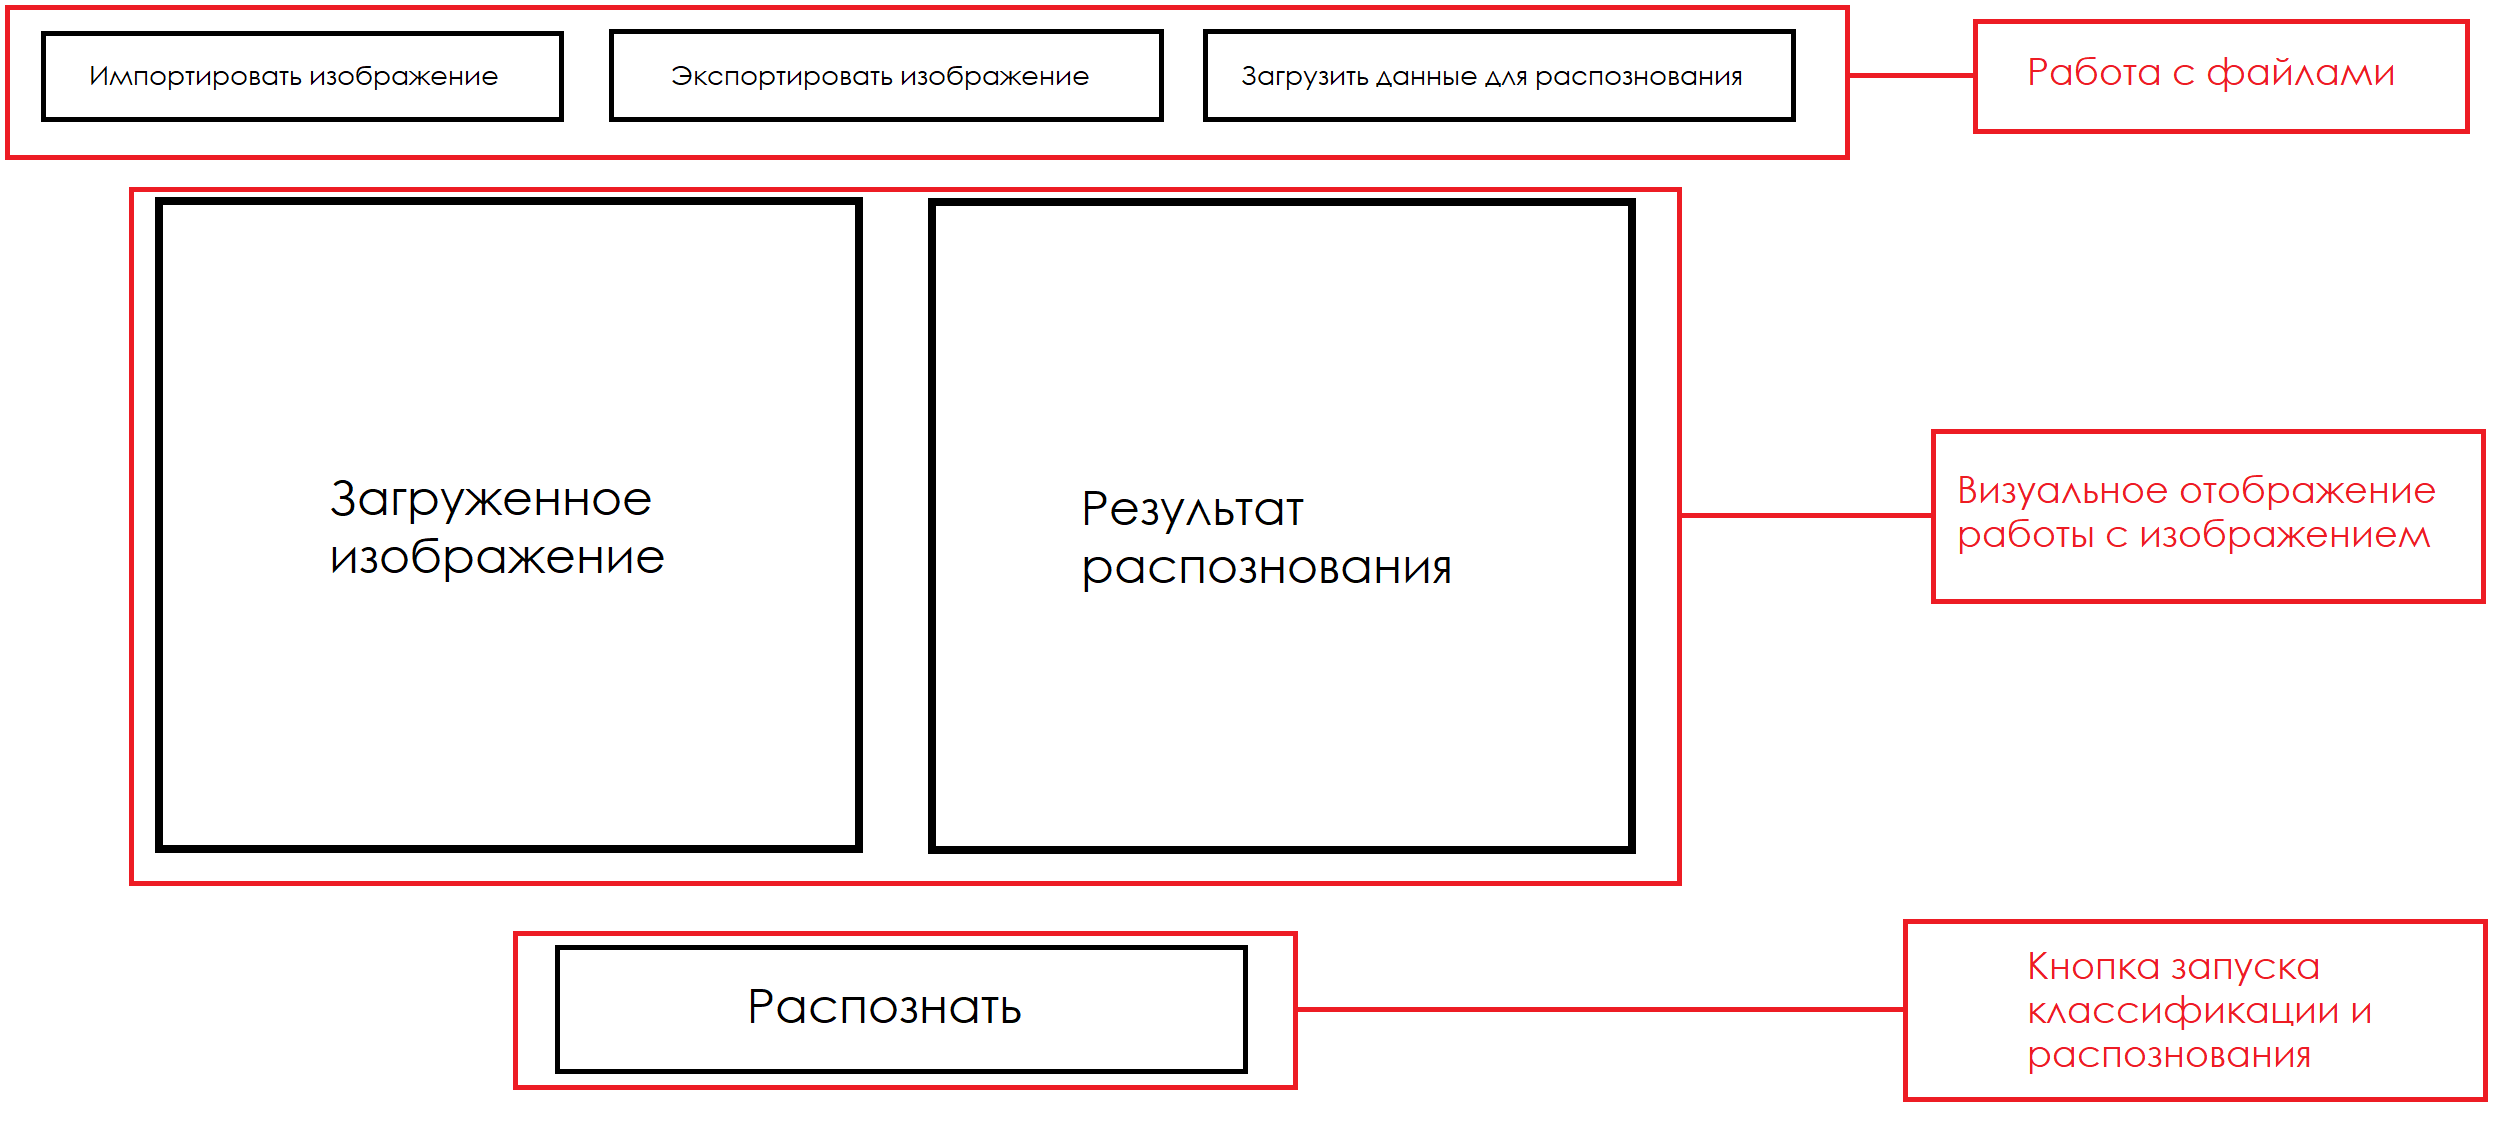
\includegraphics[width=1\linewidth]{shablon}
\caption{Композиция шаблона программы. Окно №1.}
\label{shablon:image}
\end{figure}

\begin{figure}[H]
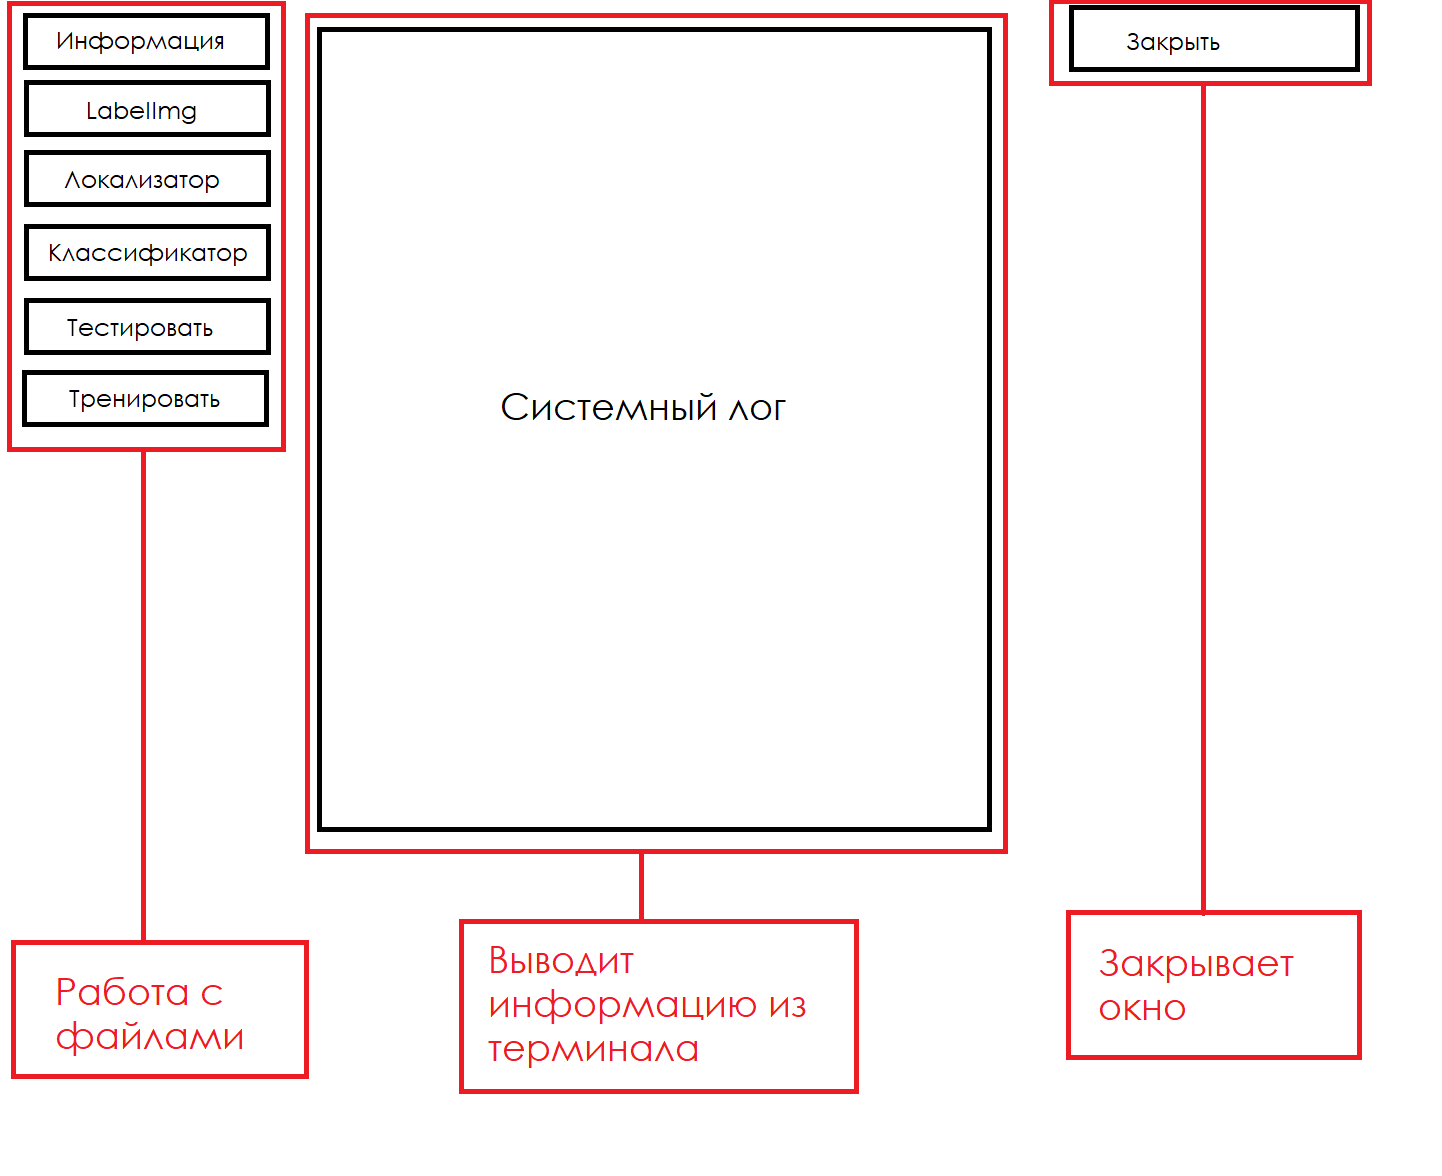
\includegraphics[width=1\linewidth]{shablon2}
\caption{Композиция шаблона программы. Окно №2.}
\label{shablon2:image}
\end{figure}

%\vspace{-\figureaboveskip} % двойной отступ не нужен (можно использовать, если раздел заканчивается картинкой)
\subsection{Моделирование вариантов использования}

Для разрабатываемого приложения была реализована модель, которая обеспечивает наглядное представление вариантов использования приложения.

Она помогает в физической разработке и детальном анализе взаимосвязей объектов. При построении диаграммы вариантов использования применяется унифицированный язык визуального моделирования UML.

Диаграмма вариантов использования описывает функциональность разрабатываемой системы. Она отражает взаимодействие системы с актерами, такими как операторы БПЛА, службы реагирования и специалисты. Каждый прецедент на диаграмме описывает действия системы для актеров: загрузка изображения, загрузка данных для распознавания, само распознавание и вывод результирующего изображения. Диаграмма обеспечивает понимание целей системы, выявляя пробелы и соответствие потребностям заинтересованных сторон. Прецедент служит для описания набора действий, которые система предоставляет пользователю.

Диаграмма предоставлена на рисунке ~\ref{actorusing:image}

\begin{figure}[H]

\includegraphics[width=1\linewidth]{actorusing}
\caption{Диаграмма вариантов использования}
\label{actorusing:image}
\end{figure}

На основании анализа предметной области в программе должны быть реализованы следующие прецеденты: 
\begin{enumerate}
	\item Распознание объекта (возгорания) на изображении с помощью нейронной сети.
	\item Сохранение результатов обучения для дальнейшего использования.
	\item Загрузка результатов обучения для дальнейшего использования.
	\item Обучение и переобучение нейронной сети.
	\item Сохранение записей для обучения нейронной сети.
\end{enumerate}

\subsection{Требования к оформлению документации}

Разработка программной документации и программного изделия должна производиться согласно ГОСТ 19.102-77 и ГОСТ 34.601-90. Единая система программной документации.

\section{Технический проект}
\subsection{Общая характеристика организации решения задачи}

Целью этого проекта является спроектировать и разработать приложение, которое поможет специализированным службам по тушению всеразличных возгораний вести более эффективную и проработанную деятельность.

Это приложение представляет собой интеллектуальную систему, предназначеную для автоматического обнаружения и классификации очагов возгораний. Эта система способна, при помощи нейронной сети, распознавать объекты, такие как возгорания и пожары, и определять их класс и уровень опасности на основе цветовых характеристик и наличиии задымленности на изображении, а также обучаться при помощи пользователя.

\subsection{Обоснование выбора технологии проектирования}

Для задачи классификации возгораний, полученных с БПЛА, используется две сверточных нейроных сетей. Такие сети хорошо подходят для задачи обработки изображений и классификации объектов, что делает их эффективным выбором для анализа данных с камер БПЛА. Она способна извлекать характерные признаки из изображений, таких как формы, текстуры и цвета, что позволяет эффективно классифицировать возгорания.

\subsubsection{Описание используемых технологий и языков программирования}

В процессе разработки приложения используются программные средства и языки программирования. Каждое программное средство и каждый язык программирования применяется для круга задач, при решении которых они необходимы.

\subsubsection{Сверточные нейронные сети}

Convolutional neural network(CNN) или Сверточная нейронная сеть - это тип искусственной нейронной сети, который широко используется для задач обработки изображений и компьютерного зрения. Ключевой особенностью CNN является использование сверточных слоев, которые извлекают характерные признаки из входных изображений. Эти признаки могут включать в себя формы, текстуры, края или цвета.

Основная идея CNN заключается в применении сверточных фильтров к входному изображению, что позволяет выявить повторяющиеся шаблоны или признаки. Эти фильтры скользят по изображению, извлекая информацию на разных уровнях абстракции. Затем эта информация проходит через дополнительные слои, такие как подвыборка или пулинг, которые уменьшают пространственные размеры данных, и полностью подключенные слои, которые выполняют классификацию или регрессию.

CNN показали впечатляющие результаты в задачах классификации изображений, обнаружения объектов, сегментации и даже в анализе медицинских изображений. Они эффективно обрабатывают большие объемы данных, обучаясь выявлять сложные зависимости и характерные признаки.

\subsubsection{Машинное обучение}

Машинное обучение - это раздел искусственного интеллекта, который фокусируется на разработке алгоритмов и моделей, позволяющих компьютерам обучаться и улучшать свои задачи без явного программирования.

Применение алгоритмов машинного обучения лежит в основе нашей системы анализа и классификации данных. Мы обучаем нашу модель на обширной базе изображений, позволяя системе эффективно распознавать и классифицировать объекты в реальном времени. Этот процесс включает в себя использование сложных алгоритмов, которые могут извлекать и интерпретировать характерные особенности из данных изображений.

\subsubsection{Язык программирования Python}

Python является одним из самых популярных и широко используемых языков программирования для разработки приложений искусственного интеллекта и машинного обучения. Он имеет простой и понятный синтаксис, что ускоряет процесс разработки и делает код более читаемым.

\subsubsection{Библиотеки Python}

\begin{itemize}
\item NumPy - фундаментальная библиотека для научных расчетов в Python. Она обеспечивает эффективную работу с многомерными массивами и матричными вычислениями, что критически важно для обработки и манипуляции данными.
\item Matplotlib - библиотека для визуализации данных. Она позволяет создавать настраиваемые и интуитивно понятные графики, диаграммы и изображения, что облегчает визуальный анализ данных и представление результатов.
\item OpenCV (Open Source Computer Vision Library) - библиотека компьютерного зрения, которая предлагает широкий спектр алгоритмов для обработки изображений и видео. Она идеально подходит для задач обработки изображений, обнаружения объектов и анализа видео, полученных с камер БПЛА.
\item Pandas - библиотека для анализа и манипуляции данными. Она предоставляет удобные структуры данных, такие как DataFrame, и богатый набор инструментов для обработки, фильтрации и агрегации данных, упрощая подготовку и анализ больших наборов данных.
\item TensorFlow - это открытая платформа машинного обучения с масштабируемыми инструментами для обучения и развертывания моделей. Она обеспечивает гибкую и эффективную инфраструктуру для создания сложных нейронных сетей. Keras - это высокоуровневый API, построенный на TensorFlow, который упрощает процесс создания и обучения нейронных сетей. Он предлагает простой и интуитивно понятный интерфейс, позволяя быстро разрабатывать и экспериментировать с различными архитектурами моделей.
\end{itemize}

\subsubsection{Архитектура сверточной нейронной сети}

Архитектура сверточной нейронной сети включает в себя 14 слоев с различными функциями.

Схема архитектуры нейронной сети представлена на рисунке ~\ref{archNC:image}.

\begin{figure}[H]
\center{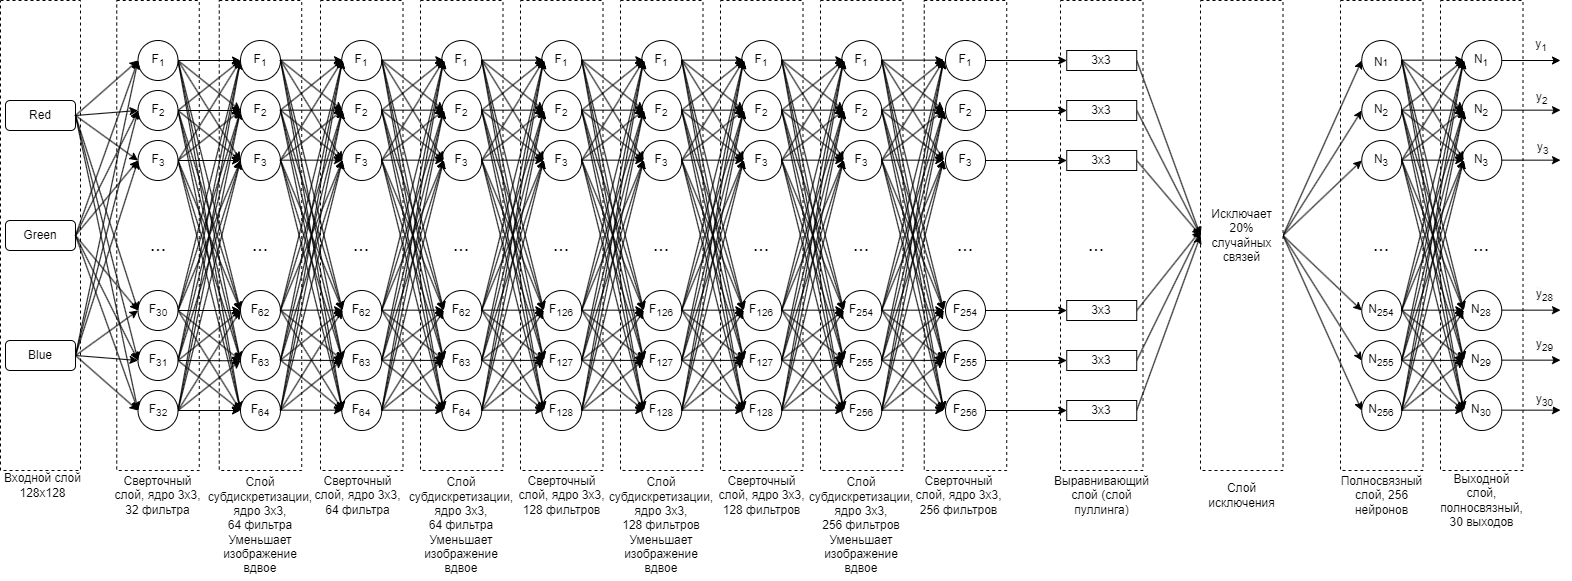
\includegraphics[width=1\linewidth]{archNC}}
\caption{Архитектура нейронной сети}
\label{archNC:image}
\end{figure}

Слои нейронной сети классификации описаны далее:

\begin{enumerate}
\item Input Layer (Входной слой)

Функция Input определяет входной слой с размером изображения 128×128 пикселей и 3 цветовыми каналами (RGB).
\item Convolutional Layers (Сверточные слои, 9)

Первый свёрточный слой Conv2D имеет 32 фильтра размером 3×3, функцию активации ReLU и параметр padding='same', который сохраняет размерность входного изображения.

Второй свёрточный слой Conv2D увеличивает количество фильтров до 64 и применяет шаг (strides) равный 2, что уменьшает размерность изображения вдвое.

Следующие два слоя Conv2D также имеют 64 фильтра и один из них снова применяет шаг 2 для уменьшения размерности.

Пятый и шестой свёрточные слои Conv2D содержат 128 фильтров каждый, с шагом 2 на шестом слое.

Седьмой свёрточный слой Conv2D сохраняет 128 фильтров и размерность.

Восьмой и девятый свёрточные слои Conv2D увеличивают количество фильтров до 256, с шагом 2 на восьмом слое.
\item Flatten Layer (Выравнивающий слой)

Слой Flatten преобразует многомерный тензор свёрточных слоёв в одномерный, чтобы его можно было подать на полносвязные слои.
\item Dropout Layer (Слой исключения)

Слой Dropout с параметром 0.2 предотвращает переобучение, случайным образом "выключая" 20% нейронов на каждом шаге обучения.
\item Dense Layers (Полносвязные слои, 2)

Первый полносвязный слой Dense имеет 256 нейронов и функцию активации ReLU.

Второй полносвязный слой Dense формирует выходной слой с 30 нейронами, количество которых соответствует количеству выходных значений, которые должна предсказывать модель.
\end{enumerate}

\subsubsection{Функция активации ReLU}

ReLU, или Rectified Linear Unit, — это функция активации, которая используется в нейронных сетях для увеличения нелинейности. 
Формула ReLU предоставлена формулой ~\ref{form0:equation}.

\begin{equation}
    \fontsize{17}{20}{f(x)=max(0,x)}
    \label{form0:equation}
\end{equation}

Это означает, что если вход x положительный, то функция возвращает x, а если x отрицательный, то функция возвращает 0. 
ReLU популярна потому, что она ускоряет обучение нейронных сетей без значительной потери точности. Она также помогает решить проблему исчезающего градиента, так как производная для положительных значений всегда равна 1, что обеспечивает более быстрое и эффективное обучение.

График функции ReLu предоставлен на изображении  ~\ref{relu:image}.

\begin{figure}[H]
\center{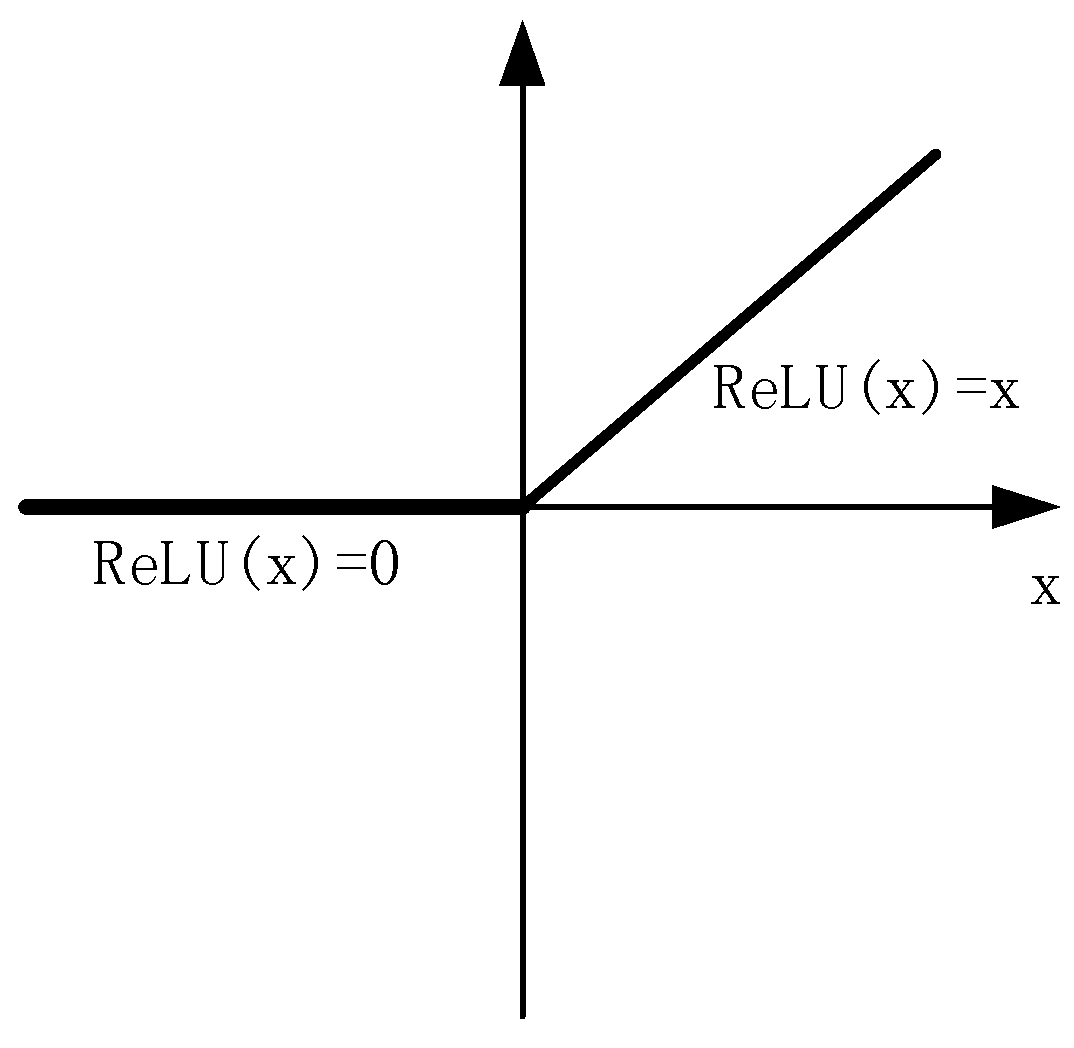
\includegraphics[width=1\linewidth]{relu}}
\caption{График функции ReLU}
\label{relu:image}
\end{figure}

\subsubsection{Функция IoU Loss}
Intersection over Union (IoU) является метрикой, используемой для измерения точности объектного детектора на определенном наборе данных. Если мы работаем с задачами компьютерного зрения, такими как сегментация изображений или обнаружение объектов, IoU может помочь оценить, насколько предсказанные границы объекта соответствуют истинным границам.

Наглядным образом функцию можно увидеть на изображении ~\ref{iou:image}.

\begin{figure}[H]
\center{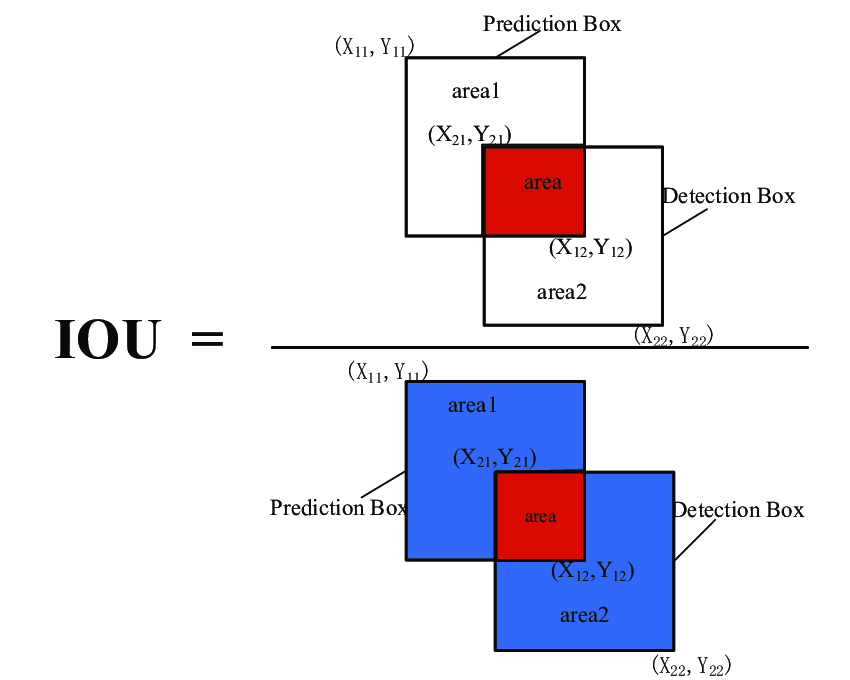
\includegraphics[width=1\linewidth]{iou}}
\caption{График функции IoU}
\label{iou:image}
\end{figure}

IoU рассчитывается по формуле ~\ref{form1:equation}.

\begin{equation}
    \fontsize{17}{20}{IoU= \frac{\text{площадь объединения}}{\text{площадь пересечения}}}
    \label{form1:equation}
\end{equation}

Где:
\begin{itemize}
\item Площадь пересечения - это область, где предсказанная граница и истинная граница объекта перекрываются.
\item Площадь объединения - это область, покрытая как предсказанной границей, так и истинной границей, вместе взятых.
\end{itemize}

IoU loss - это функция потерь, которая используется для обучения моделей, выполняющих задачи, связанные с локализацией объектов. Вместо того чтобы использовать стандартные функции потерь, такие как кросс-энтропия, которые могут не полностью отражать точность локализации, IoU loss напрямую оптимизирует метрику IoU, стремясь увеличить площадь пересечения и уменьшить площадь объединения.

Функция потерь IoU показана в формуле ~\ref{form2:equation}.

\begin{equation}
	\fontsize{17}{20}{IoU loss=1−IoU}
	\label{form2:equation}
\end{equation}

Таким образом, минимизация IoU loss в процессе обучения приводит к увеличению IoU между предсказанными и истинными границами, что помогает в задаеч локализации объектов нашего проекта.

\subsection{Диаграмма компонентов}

Диаграмма компонентов представляет структуру системы в виде набора компонентов и их взаимосвязей. Каждый компонент отвечает за определенную функцию в рамках системы и может включать в себя подсистемы или модули.

\begin{itemize}
\item Графический интерфейс: отвечает за создание интерфейса, в котором пользователь наглядно видит результат распознования в сравнении с оригиналом;
\item Обработка изображения: включает в себя методы улучшения качества изображений, такие как коррекция освещения, удаление шумов и извлечение важных признаков;
\item Сверточная нейронная сеть (CNN): Ядро этой системы, реализующее алгоритмы обучения и распознавания объектов;
\item Данные параметров нейронной сети: представляют собой обученную модель, которая хранит в себе веса и параметры, извлеченные из данных во время процесса обучения;
\item Классификация объекта: этот модуль используется для классификации возгорания;
\item Генерация отчета: отвечает за создание отчета для выведения класса возгорания и оценки его опасности.
\end{itemize}

\subsubsection{Взаимодействие компонентов}

\begin{enumerate}
\item Пользователь загружает изображение через графический интерфейс пользователя.
\item Интерфейс передает изображение в модуль обработки изображения.
\item После обработки данные передаются в модуль сверточной нейронной сети для распознавания объекта.
\item Модуль данных параметров передает веса и параметры и корректирует работу нейронной сети.
\item Результаты распознавания классифицируются в модуле классификации объекта.
\item Модуль генерации отчета выводит данные о возгорании в графическом интерфейсе.
\end{enumerate}

Диаграмма компонентов представленна на рисунке ~\ref{comp:image}.

\begin{figure}[H]
\center{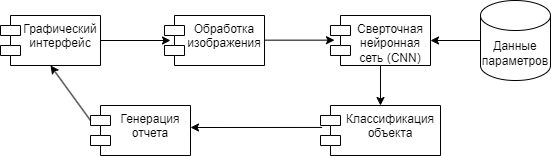
\includegraphics[width=1\linewidth]{comp}}
\caption{Диаграмма компонентов}
\label{comp:image}
\end{figure}

\subsubsection{Диаграмма программных классов}

Точкой входа в программу является класс main. В этом классе осуществляется запуск и инициализация основных компонентов программы:
\begin{itemize}
	\item dataprocessing - компонент, отвечающий за обработку данных и изображений.
	\item creatingtfrecordclassifier - компонент, отвечающий за создание и загрузку изображений и создания их записи в формате .tfrecord
	\item creatingtfrecordlocalizer - компонент, отвечающий за создание и загрузку изображений и создания их записи в формате .tfrecord
	\item classifier - компонент, отвечающий за работу с нейронной сетью по классификации данных, её обучение и тестирование.
	\item training - компонент, отвечающий за работу с нейронной сетью по распознанию данных, её обучение и тестирование.
\end{itemize}

Диаграмма классов предоставлена на рисунке ~\ref{classdiag:image}.

\begin{figure}[H]
\center{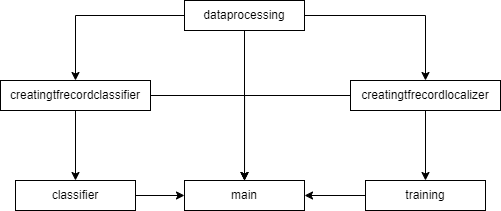
\includegraphics[width=1\linewidth]{classdiag}}
\caption{Диаграмма классов и их связей}
\label{diagclass:image}
\end{figure}

На диаграмме показаны данные связи:
\begin{itemize}
	\item Связь dataprocessing - main. Класс main использует основные функции класса dataprocessing, такие как отображение информации о изображении, загрузка изображения и нормализация координат изображения.
	\item Связь dataprocessing - creatingtfrecordclassifier. Класс creatingtfrecordclassifier использует основные функции класса dataprocessing, такие как загрузка изображения и нормализация координат изображения. Для создания записи tfrecord необходимо создать запись со всеми изображениями и файлами формата .xml.
	\item Связь dataprocessing - creatingtfrecordlocalizer. Класс creatingtfrecordlocalizer использует основные функции класса dataprocessing, такие как загрузка изображения и нормализация координат изображения. Для создания записи tfrecord необходимо создать запись со всеми изображениями и файлами формата .xml.
	\item Связь creatingtfrecordclassifier - classifier. Для работы классу classifier нужен созданный в классе creatingtfrecordclassifier файл tfrecord.
	\item Связь creatingtfrecordclassifier - main.  Класс main использует основные функции класса creatingtfrecordclassifier, такие как создание файла tfrecord для классификатора.
	\item Связь creatingtfrecordlocalizer - training. Для работы классу training нужен созданный в классе creatingtfrecordlocalizer файл tfrecord.
	\item Связь creatingtfrecordlocalizer - main.  Класс main использует основные функции класса creatingtfrecordlocalizer, такие как создание файла tfrecord для локализатора.
	\item Связь classifier - main. Класс main использует основные функции класса classifier, такие как тестирование, обучение, загрузка и сохранение сети.
	\item Связь localizer - main. Класс main использует основные функции класса localizer, такие как тестирование, обучение, загрузка и сохранение сети.
\end{itemize}


\subsection{ Проектирование пользовательского интерфейса}
%  накинуть ссылок на литературу
На основании требований к пользовательскому интерфейсу, представленных в пункте 2.3 технического задания, был разработан графический интерфейс приложения. Для создания пользовательского интерфейса используется библеотека tkinter и matlibplot.

На рисунке ~\ref{maketinterface:image} представлен макет интерфейса окон для распознания и обучения нейронной сети. Данный макет содержит следующие элементы:
\begin{enumerate}
\item Загрузка изображения из системы.
\item Загрузка своей модели нейронной сети.
\item Запустить распознание изображения
\item Открыть окно тренировки модели нейронной сети.
\item Поле загруженного изображения.
\item Поле изображения с распознанным возгоранием.
\item Закрывает окно тренировки модели нейронной сети.
\item Показывает информацию о первой картинке в папке с изображениями для обучения.
\item Запускает стороннюю программу labelimg.
\item Показывает в поле для вывода информацию о наличии файлов.
\item Создает новую запись tfrecord для локализатора.
\item Создает новую запись tfrecord для классификатора.
\item Запускает функцию тестирования классификатора.
\item Запускает другую функцию тестриования классификатора с точными значениями.
\item Запускает функцию обучения классификатора.
\item Сохраняет модель нейронной сети классификатора.
\item Сохраняет модель нейронной сети локализатора.
\item Загружает модель нейронной сети локализатора.
\item Запускает функцию тестирования нейронной сети локализатора.
\item Запускает функции для обучения нейронной сети локализатора.
\item Поле вывода информации из терминала после выполнения любых операций.
\end{enumerate}

\begin{figure}[H]
\center{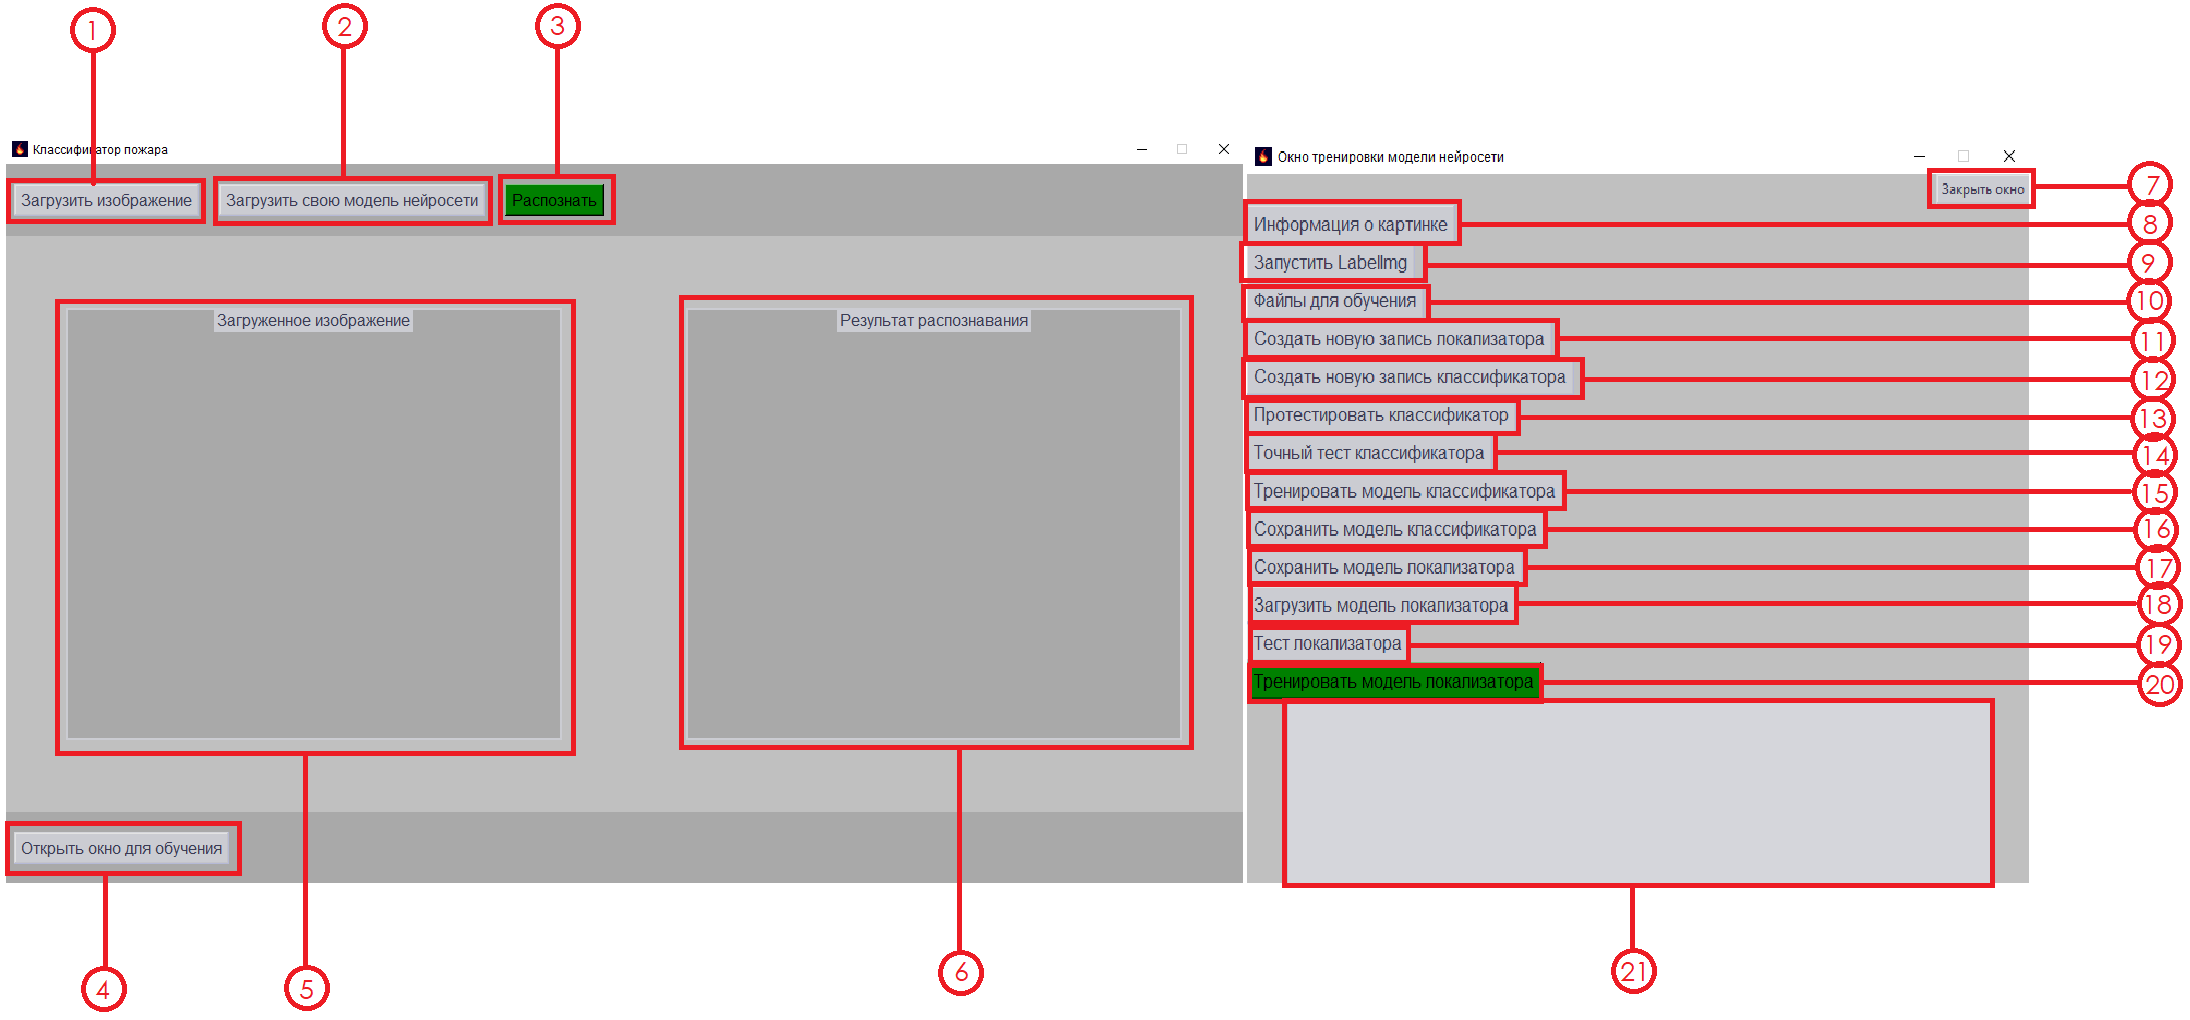
\includegraphics[width=1\linewidth]{maketinterface}}
\caption{Макет интерфейса окна распознавания и окна обучения нейронной сети}
\label{maketinterface:image}
\end{figure}

















\ifПрактика{}\else{
   \section{Рабочий проект}
\subsection{Классы, используемые при разработке приложения}

Список классов и методов, которые были использованы при создании приложения представлены далее.

\subsubsection{Класс main}

Класс main явлаяется точкой входа в приложение и используется для реализации идентификации объектов с помощью нейронной сети. Здесь происходит инициализация основных компонентов программы в качестве кнопок на интерфейсе приложения. 
Описание полей и методов данного класса представлено в таблице \ref{classmain:table}.

\renewcommand{\arraystretch}{0.8} % уменьшение расстояний до сетки таблицы
\begin{xltabular}{\textwidth}{|X|p{1.5cm}|>{\setlength{\baselineskip}{0.7\baselineskip}}p{2.85cm}|>{\setlength{\baselineskip}{0.7\baselineskip}}p{4.85cm}|}
\caption{Спецификация полей класса <<main>> \label{classmain:table}}\\
\hline \centrow \setlength{\baselineskip}{0.7\baselineskip} Наименование& \centrow \setlength{\baselineskip}{0.7\baselineskip} Метод доступа & \centrow Тип данных & \centrow Описание \\
\hline \centrow 1 & \centrow 2 & \centrow 3 & \centrow 4\\ 
\hline
\endfirsthead
\caption*{Продолжение таблицы \ref{classmain:table}}\\
\hline \centrow 1 & \centrow 2 & \centrow 3 & \centrow 4\\ 
\hline
\finishhead
path\_for\_one & public & String & Хранит путь к выбранному изображению\\
\hline localizator & public & tf.keras.Model & Модель локализатора, загруженная из файла. Файл хранится в корневой папке проекта и создается в классе training. \\
\hline classifier & public & tf.keras.Model & Модель классификатора, загруженная из файла. Файл хранится в корневой папке проекта и создается в классе cllassifier. \\
\hline window & private & Tk & Главное окно приложения. Окно настроено и имеет несколько вложений соответсвтующие визуальной составляющей. Содержит в себе кнопки и поля Canvas. \\
\hline image\_field\_raw & private & Canvas & Холст для отображения исходного изображения. Содержится в окне window. \\
\hline image\_field\_ready & private & Canvas & Холст для отображения результата распознавания. Содержится в окне window. \\
\hline ConsoleRedirector & public & Class & Класс для перенаправления вывода консоли в текстовое поле text с помощью функции sys.stdout = ConsoleRedirector(text). \\
\hline image\_field\_ready & private & Canvas & Холст для отображения результата распознавания. Содержится в окне window. \\
\hline detect\_objects & private & Function & Функция для обнаружения объектов на изображении с использованием модели локализатора. Здесь происходит подготовка изображения, локализация, нормализация, разделение на элементы, нарезание изображений и сбор в массив (10, 32, 32, 3). Далее происходит классификация, счет метки класса и сбор координат в нормальный вид. \\
\hline namespace & public & Dictionary & Словарь для сопоставления индексов классов с их названиями. В нашем варианте 0 - Ничего (nothing), 1- Возгорание (fire). \\
\hline visualize & private & Function & Функция для визуализации результатов детекции с помощью OpenCV. Рисует текст и квадраты на изображении в соответствии с распознанными объектами (возгораниями) \\
\hline prettify & private & Function & Функция для улучшения результатов детекции путём объединения перекрывающихся рамок. Здесь вычисляем IoU, самый надежный способ определить совпадение. И если ни с чем не обьединили, так и оставляем результат. \\
\hline detect\_fire\_in\_image & private & Function & Функция для обнаружения огня на изображении и его визуализации. Считывает изображение, переводит его в matplotlib и выводит на Canvas поле результата. \\
\hline loadimage & public & Function & Функция для загрузки изображения через диалоговое окно. Также помещает его в Canvas поле загруженного изображения. \\
\hline detect & private & Function & Функция для запуска процесса обнаружения огня на загруженном изображении. Вызывает detect\_fire\_in\_image(). \\
\hline check\_and\_install\_packages & private & Function & Функция для проверки и установки необходимых пакетов PyQt5 и sip. Вызывается для предварительного устранения ошибок с пакетами при запуске labelimg. \\
\hline run\_labelimg & private & Function & Функция для запуска приложения LabelImg для аннотации изображений. Labelimg установлен заранее, но требует для запуска дополнительные пакеты в системе. \\
\hline create\_tfrec\_classifier & private & Function & Функция для создания TFRecord для классификатора. Вызывает функцию из другого класса. \\
\hline start\_train\_localizer & private & Function & Функция для начала обучения модели локализатора. Вызывает функцию train() и loadmodel() из другого класса. \\
\hline train\_window\_open & private & Function & Открывает новое окно для обучения нейронной сети. Здесь реализованы функции для удобного обучения, тестирования и работы с файлами нейронной сети. \\
\hline load\_model\_data & private & Function & Функция для загрузки пользовательской модели нейросети.
\end{xltabular}
\renewcommand{\arraystretch}{1.0} % восстановление сетки

\subsubsection{Класс dataprocessing}

Класс dataprocessing отвечает за обработку данных и изображений. Класс предназначен для обработки данных из XML файла, который содержит аннотации для изображений, используемых в наших задачах. В классе парсится XML файл, извлекается информацию о размеченных объектах и их координатах, загружается соответствующее изображение и визуализирует его. 
Описание полей и методов данного класса представлено в таблице \ref{classdataprocessing:table}.

\renewcommand{\arraystretch}{0.8} % уменьшение расстояний до сетки таблицы
\begin{xltabular}{\textwidth}{|X|p{2.5cm}|>{\setlength{\baselineskip}{0.7\baselineskip}}p{4.85cm}|>{\setlength{\baselineskip}{0.7\baselineskip}}p{4.85cm}|}
\caption{Спецификация полей класса <<dataprocessing>> \label{classdataprocessing:table}}\\
\hline \centrow \setlength{\baselineskip}{0.7\baselineskip} Наименование& \centrow \setlength{\baselineskip}{0.7\baselineskip} Метод доступа & \centrow Тип данных & \centrow Описание \\
\hline \centrow 1 & \centrow 2 & \centrow 3 & \centrow 4\\ \hline
\endfirsthead
\caption*{Продолжение таблицы \ref{classdataprocessing:table}}\\
\hline \centrow 1 & \centrow 2 & \centrow 3 & \centrow 4\\ \hline
\finishhead
tree & public & xml.etree.ElementTree & Объект дерева XML, содержащий структурированные данные из файла XML. Значением является адрес файла для информирования. \\ 
\hline root & public & xml.etree.ElementTree & Корневой элемент XML файла, предоставляющий доступ к дочерним элементам. Парсинг.\\ 
\hline num\_objects & public & int & Количество объектов, размеченных в XML файле. Количество размеченных объектов (6 - кол-во служебных элементов, таких как размер, название и т.д)\\ 
\hline load\_img & public & Function & Функция для загрузки и предобработки изображения с использованием TensorFlow. \\ 
\hline cords & public & list & Список для хранения нормализованных координат объектов. \\ 
\hline w & public & int & Ширина изображения, извлеченная из XML файла. \\ 
\hline h & public & int & Высота изображения, извлеченная из XML файла. \\ 
\hline object\_cords & public & list & Список для хранения нормализованных координат одного объекта. Тут мы также нормализуем координаты от -1 до 1, опираясь на исходные координаты. \\ 
\hline img & public & Tensor & Тензор изображения после загрузки и предобработки. \\ 
\hline plt.figure & public & Function & Функция для создания новой фигуры в Matplotlib. \\ 
\hline plt.subplot & public & Function & Функция для добавления подграфика в текущую фигуру. \\ 
\hline plt.imshow & public & Function & Функция для отображения изображения в подграфике.  \\ 
\hline plt.axis & public & Function & Функция для управления отображением осей графика. \\ 
\hline plt.show & public & Function & Функция для отображения всей фигуры с подграфиками. Открывает окно с исходным изображением. \\
\end{xltabular}
\renewcommand{\arraystretch}{1.0} % восстановление сетки

\subsubsection{Класс creatingtfrecordclassifier}

Класс creatingtfrecordclassifier отвечает за создание и загрузку изображений и создания их записи в формате .tfrecord. В этом классе подготавливаются данные для дальнейшего использования в других классах и главное - создание файла classifier\_dataset.tfrecord . 
Описание полей и методов данного класса представлено в таблице \ref{classtfrecordclassifier:table}.

\renewcommand{\arraystretch}{0.8} % уменьшение расстояний до сетки таблицы
\begin{xltabular}{\textwidth}{|X|p{1.5cm}|>{\setlength{\baselineskip}{0.7\baselineskip}}p{2.85cm}|>{\setlength{\baselineskip}{0.7\baselineskip}}p{3.85cm}|}
\caption{Спецификация полей класса <<creatingtfrecordclassifie>> \label{classtfrecordclassifier:table}}\\
\hline \centrow \setlength{\baselineskip}{0.7\baselineskip} Наименование& \centrow \setlength{\baselineskip}{0.7\baselineskip} Метод доступа & \centrow Тип данных & \centrow Описание \\
\hline \centrow 1 & \centrow 2 & \centrow 3 & \centrow 4\\ \hline 
\endfirsthead
\caption*{Продолжение таблицы \ref{classtfrecordclassifier:table}}\\
\hline \centrow 1 & \centrow 2 & \centrow 3 & \centrow 4\\ \hline
\finishhead
fn & public & str & Путь к папке с изображениями. Значением является адрес папки с нашими изображениями и xml файлами.\\ 
\hline check\_xml\_list & public & function & Функция для создания списка XML файлов в указанной папке. Формируем список всех xml файлов в папке.\\ 
\hline load\_img & public & function & Функция для загрузки и предобработки изображения. \\ 
\hline create\_load\_tfrec\_for\_classifier & public & function & Функция для создания TFRecord для классификатора. Здесь мы преобразуем папку в tfrecord для классификарора\\ 
\hline namespace & public & dictionary & Словарь для сопоставления названий с метками классов. В нашем случае 0 - Ничего (nothing), 1- Возгорание (fire). \\ 
\hline saveinrecord & public & function & Внутренняя функция для сохранения обработанного изображения и метки в TFRecord. Создается запись writer, данные предоставляются в байтовом виде и собирается экземляр, который потом записывается в запись writer.\\ 
\hline parse\_record & public & function & Функция для разбора записей TFRecord. Имена элементов остаются как при записи
\end{xltabular}
\renewcommand{\arraystretch}{1.0} % восстановление сетки

\subsubsection{Класс creatingtfrecordlocalizer}

Класс creatingtfrecordlocalizer отвечает за создание и загрузку изображений и создания их записи в формате .tfrecord. В этом классе подготавливаются данные для дальнейшего использования в других классах и главное - создание файла localizer\_dataset.tfrecord . 
Описание полей и методов данного класса представлено в таблице \ref{classtfrecordlocalizer:table}.

\renewcommand{\arraystretch}{0.8} % уменьшение расстояний до сетки таблицы
\begin{xltabular}{\textwidth}{|X|p{1.5cm}|>{\setlength{\baselineskip}{0.7\baselineskip}}p{3cm}|>{\setlength{\baselineskip}{0.7\baselineskip}}p{3.85cm}|}
\caption{Спецификация полей класса <<creatingtfrecordlocalizer>> \label{classtfrecordlocalizer:table}}\\
\hline \centrow \setlength{\baselineskip}{0.7\baselineskip} Наименование& \centrow \setlength{\baselineskip}{0.7\baselineskip} Метод доступа & \centrow Тип данных & \centrow Описание \\
\hline \centrow 1 & \centrow 2 & \centrow 3 & \centrow 4\\ \hline
\endfirsthead
\caption*{Продолжение таблицы \ref{classtfrecordlocalizer:table}}\\
\hline \centrow 1 & \centrow 2 & \centrow 3 & \centrow 4\\ \hline
\finishhead
fn & public& string & Путь к папке с изображениями. Значением является адрес папки с нашими изображениями и xml файлами. \\ 
\hline load\_img & private & function & Загружает изображение, декодирует, нормализует и изменяет размер. \\ 
\hline create\_load\_tfrec\_for\_localizer & private & function & Создает TFRecord для локализатора из XML файлов. \\ 
\hline p & private & list & Формируем список всех xml файлов в папке. \\ 
\hline writer & private & TFRecordWriter & Записывает данные в TFRecord. Создание самой записи \\ 
\hline tree & private & ElementTree & Адрес файла \\ 
\hline root & private & Element & Парсит XML файлы. \\ 
\hline num\_objects & private & int & Количество объектов в XML файле. \\ 
\hline cords & private & list & Список координат объектов. \\ 
\hline w & private & int & Ширина изображения. \\
 \hline h & private & int & Высота изображения. \\ 
 \hline object\_cords & private & list & Координаты одного объекта. Тут мы также нормализуем координаты от -1 до 1, опираясь на исходные координаты. \\ 
 \hline img & private & Tensor & Тензор изображения. \\ 
 \hline serialized\_img & private & bytes & Сериализованное изображение. Готовим данные, представляем в байтовом виде.\\ 
 \hline serialized\_cords & private & bytes & Сериализованные координаты. Готовим данные, представляем в байтовом виде.\\ 
 \hline example & private & Example & Пример данных для TFRecord. Собираем экзепмляр\\ 
 \hline dataset & private & TFRecordDataset & Набор данных из TFRecord. Сразу после создания проверка чтения записи. \\ 
 \hline parse\_record & private & function & Разбирает запись из TFRecord. Имена элементов как при записи\\ 
 \hline feature\_description & private & dict & Описание приходящего экземпляра. \\ 
 \hline parsed\_record & private & dict & Разобранный экземпляр. 
\end{xltabular}
\renewcommand{\arraystretch}{1.0} % восстановление сетки

\subsubsection{Класс classifier}

Класс classifier отвечает за работу с нейронной сетью по классификации данных, её обучение и тестирование. В этом классе  реализован парсинг элементов из tfrecord, загрузка и создание модели нейросети, а также построение её архитектуры.
Описание полей и методов данного класса представлено в таблице \ref{classifier:table}.

\renewcommand{\arraystretch}{0.8} % уменьшение расстояний до сетки таблицы
\begin{xltabular}{\textwidth}{|X|p{1.5cm}|>{\setlength{\baselineskip}{0.7\baselineskip}}p{2.85cm}|>{\setlength{\baselineskip}{0.7\baselineskip}}p{4.85cm}|}
\caption{Спецификация полей класса <<classifier>> \label{classifier:table}}\\
\hline \centrow \setlength{\baselineskip}{0.7\baselineskip} Наименование& \centrow \setlength{\baselineskip}{0.7\baselineskip} Метод доступа & \centrow Тип данных & \centrow Описание \\
\hline \centrow 1 & \centrow 2 & \centrow 3 & \centrow 4\\ \hline
\endfirsthead
\caption*{Продолжение таблицы \ref{classifier:table}}\\
\hline \centrow 1 & \centrow 2 & \centrow 3 & \centrow 4\\ \hline
\finishhead
\hline parse\_record & public & function & Разбирает запись TFRecord, возвращая изображение и имя. \\ 
\hline shuffle, cache, prefetch, batch & public & method & Подготавливает датасет к обучению: перемешивание, кэширование, предварительная загрузка, батчинг. \\ 
\hline test\_classifier & public & function & Визуализирует примеры из датасета и их метки. \\ 
\hline Model & public & class & Определяет модель нейросети с методами для обучения. \\ 
\hline training\_step & public & method & Выполняет шаг обучения, возвращая среднее значение потерь. \\ 
\hline trainclass & public & function & Обучает классификатор и визуализирует диаграмму потерь. \\ 
\hline imshow\_and\_pred & public & function & Визуализирует изображения и предсказания модели с помощью matplotlib. \\ 
\hline saveclassifier & public & function & Сохраняет обученную модель классификатора.
\end{xltabular}
\renewcommand{\arraystretch}{1.0} % восстановление сетки


\subsubsection{Класс training}

Класс training отвечает за работу с нейронной сетью по локализации данных, её обучение и тестирование. В этом классе  реализован парсинг элементов из tfrecord, загрузка и создание модели нейросети, а также построение её архитектуры и явное обучение.
Описание полей и методов данного класса представлено в таблице \ref{localizer:table}.

\renewcommand{\arraystretch}{0.8} % уменьшение расстояний до сетки таблицы
\begin{xltabular}{\textwidth}{|X|p{1.5cm}|>{\setlength{\baselineskip}{0.7\baselineskip}}p{2.85cm}|>{\setlength{\baselineskip}{0.7\baselineskip}}p{4.85cm}|}
\caption{Спецификация полей класса <<training>> \label{localizer:table}}\\
\hline \centrow \setlength{\baselineskip}{0.7\baselineskip} Наименование& \centrow \setlength{\baselineskip}{0.7\baselineskip} Метод доступа & \centrow Тип данных & \centrow Описание \\
\hline \centrow 1 & \centrow 2 & \centrow 3 & \centrow 4\\ \hline
\endfirsthead
\caption*{Продолжение таблицы \ref{localizer:table}}\\
\hline \centrow 1 & \centrow 2 & \centrow 3 & \centrow 4\\ \hline
\finishhead
parse\_record & public & function & Разбирает запись TFRecord, возвращая изображение и координаты. \\
\hline IoU\_Loss & public & function & Вычисляет потери IoU между истинными и предсказанными рамками. \\
\hline Model & public & class & Определяет модель нейросети с методами для обучения. \\
\hline training\_step & public & method & Выполняет шаг обучения, возвращая значение потерь. \\
\hline savemodel & public & function & Сохраняет обученную модель. \\
\hline loadmodel & public & function & Загружает веса модели. \\
\hline testing & public & function & Тестирует модель, визуализируя результаты. \\
\hline train & public & function & Обучает модель и визуализирует историю потерь.
\end{xltabular}
\renewcommand{\arraystretch}{1.0} % восстановление сетки


\subsection{Модульное тестирование разработанного приложения}

Модульные тесты для класса main из модели данных представлены на рисунках \ref{test1:image}-\ref{test3:image}.

\begin{figure}[H]
\begin{lstlisting}[language=Python]
import unittest
from main import detect_objects, visualize, prettify

class TestFireDetection(unittest.TestCase):

    def setUp(self):
        self.test_image = np.zeros((1024, 1024, 3), dtype=np.uint8)
        self.test_cords = np.array([[10, 20, 30, 40] for _ in range(10)])
        self.test_classes = np.array([1 for _ in range(10)])
        self.test_probs = np.array([0.9 for _ in range(10)])

    def test_detect_objects(self):
        cords, classes, probs = detect_objects(self.test_image)
        self.assertEqual(len(cords), 10)
        self.assertEqual(len(classes), 10)
        self.assertEqual(len(probs), 10)
        self.assertTrue((cords >= 0).all() and (cords <= 1024).all())
        self.assertTrue((classes >= 0).all() and (classes <= 1).all())
        self.assertTrue((probs >= 0).all() and (probs <= 1).all())

    def test_visualize(self):
        result_image = visualize(self.test_image, self.test_cords, self.test_classes, self.test_probs)
        self.assertIsNotNone(result_image)
        self.assertEqual(result_image.shape, self.test_image.shape)

    def test_prettify(self):
        new_cords, new_classes, new_probs = prettify(self.test_cords, self.test_classes, self.test_probs)
        self.assertIsNotNone(new_cords)
        self.assertIsNotNone(new_classes)
        self.assertIsNotNone(new_probs)
        self.assertTrue(len(new_cords) <= len(self.test_cords))
\end{lstlisting}  
\caption{Модульный тест основных методов распознавания, визуализации и объединения класса main}
\label{test1:image}
\end{figure}

\begin{figure}[H]
\begin{lstlisting}[language=Python]
import unittest
from unittest.mock import patch
from main import detect_fire_in_image, loadimage, detect

class TestFireDetection(unittest.TestCase):

    def setUp(self):
        self.test_path = 'D:/NeuroPractice/NeuroPractice/src/images/fire1.jpg'
        self.test_image = np.zeros((1024, 1024, 3), dtype=np.uint8)
        
     def test_detect_fire_in_image(self):
        result = detect_fire_in_image(self.test_path)
        self.assertIsNotNone(result)
        self.assertEqual(result.shape, (1024, 1024, 3))
    def test_loadimage(self, mock_open):
        mock_open.return_value.__enter__.return_value = 'fake file content'
        image = loadimage('fake/path/to/image.jpg')
        mock_open.assert_called_with('fake/path/to/image.jpg', 'rb')
        self.assertIsNotNone(image)

    @patch('main.detect')
    def test_detect(self, mock_detect):
        mock_detect.return_value = True
        result = detect('fake/path/to/image.jpg')
        mock_detect.assert_called_once()
        self.assertTrue(result)
\end{lstlisting}  
\caption{Модульный тест методов распознавания возгораний, загрузки изображения и вложенного метода detect класса main}
\label{test2:image}
\end{figure}

\begin{figure}[H]
\begin{lstlisting}[language=Python]
import unittest
from your_module import detect_objects
import tensorflow as tf
import numpy as np

class TestObjectDetection(unittest.TestCase):
    def test_detect_objects(self):
        test_image = np.random.randint(0, 256, (128, 128, 3), dtype=np.uint8)
        test_image = tf.convert_to_tensor(test_image, dtype=tf.float32)

        cords, classes, probs = detect_objects(test_image)

        self.assertIsInstance(cords, np.ndarray, "Координаты должны быть массивом NumPy")
        self.assertIsInstance(classes, np.ndarray, "Классы должны быть массивом NumPy")
        self.assertIsInstance(probs, list, "Вероятности должны быть списком")

        self.assertEqual(cords.shape, (10, 4), "Массив координат должен иметь форму (10, 4)")
        self.assertEqual(len(classes), 10, "Массив классов должен содержать 10 элементов")
        self.assertEqual(len(probs), 10, "Список вероятностей должен содержать 10 элементов")

        for prob in probs:
            self.assertGreaterEqual(prob, 0, "Вероятность должна быть больше или равна 0")
            self.assertLessEqual(prob, 1, "Вероятность должна быть меньше или равна 1")
\end{lstlisting}  
\caption{Отдельный модульный тест метода распознавания класса main}
\label{test3:image}
\end{figure}



\subsection{Системное тестирование разработанного приложения}
В целях проверки работоспособности программно-информационной системы было проведено системное тестирование. Описание тестов, их результаты и скриншоты экрана представлены в данном разделе.

На рисунке \ref{main:image} представлена главная страница сайта «Русатом – Аддитивные технологии».
\newpage % при необходимости можно переносить рисунок на новую страницу
\begin{figure}[H] % H - рисунок обязательно здесь, или переносится, оставляя пустоту
\center{\includegraphics[width=1\linewidth]{main1}}
\center{\includegraphics[width=1\linewidth]{main2}}
\center{\includegraphics[width=1\linewidth]{main3}}
\caption{Главная страница сайта «Русатом – Аддитивные технологии»}
\label{main:image}
\end{figure}

На рисунке \ref{systemtest1:image} представлен интерфейс программы.
\begin{figure}[H]
\centering
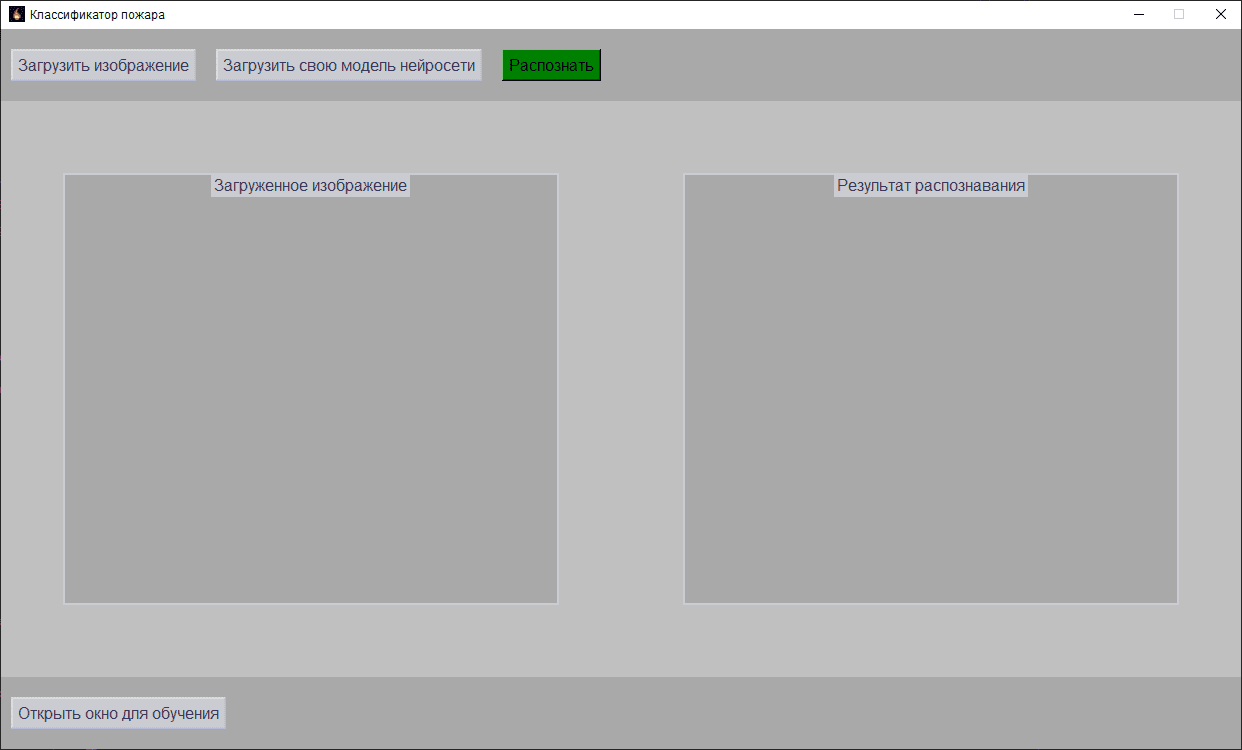
\includegraphics[width=1\linewidth]{systemtest1}
\caption{Интерфейс программы}
\label{systemtest1:image}
\end{figure}

На рисунках \ref{systemtest_responce:image}-\ref{systemtest_responce4:image} представлен полный путь распознания объекта на изображении.

\begin{figure}[H]
\center{\includegraphics[width=1\linewidth]{systemtest_responce}}
\caption{Диалоговое окно загрузки файла Машина.png}
\label{systemtest_responce:image}
\end{figure}

\begin{figure}[H]
\center{\includegraphics[width=1\linewidth]{systemtest_responce1}}
\caption{Изображение отображено в интерфейсе программы}
\label{systemtest_responce1:image}
\end{figure}

\begin{figure}[H]
\center{\includegraphics[width=1\linewidth]{systemtest_responce2}}
\caption{Окно выбора модели для распознания}
\label{systemtest_responce2:image}
\end{figure}

\begin{figure}[H]
\center{\includegraphics[width=1\linewidth]{systemtest_responce3}}
\caption{Распознанный объект отображен на интерфейсе}
\label{systemtest_responce3:image}
\end{figure}

\begin{figure}[H]
\center{\includegraphics[width=1\linewidth]{systemtest_responce4}}
\caption{Диалоговое окно сохранения результата}
\label{systemtest_responce4:image}
\end{figure}

На рисунках \ref{systemtest_train1:image}-\ref{systemtest_train3:image} представлены все варианты обучения нейронной сети.

На рисунке \ref{systemtest_train1:image} была нажата кнопка обучать, после чего открылось окно выбора набора.

\begin{figure}[H]
\center{\includegraphics[width=1\linewidth]{systemtest_train1}}
\caption{Окно выбора обучающего набора}
\label{systemtest_train1:image}
\end{figure}

После выбора нового набора появилось окно, предлагающее назвать модель и обучить её.

\begin{figure}[H]
\center{\includegraphics[width=1\linewidth]{systemtest_train2}}
\caption{Окно выбора названия новой модели}
\label{systemtest_train2:image}
\end{figure}

Вместо создания нового набора, после нажатия кнопки обучать, можно выбрать заготовленный набор и обучить нейронную сеть по нему.

\begin{figure}[H]
\center{\includegraphics[width=1\linewidth]{systemtest_train3}}
\caption{Выбор обучения по набору ''Белый''}
\label{systemtest_train3:image}
\end{figure}

На рисунке \ref{systemtest_responce5:image} было загружено изображение кошки.

\begin{figure}[H]
\center{\includegraphics[width=1\linewidth]{systemtest_responce5}}
\caption{Интерфейс с изображением кошки}
\label{systemtest_responce5:image}
\end{figure}

На рисунке \ref{systemtest_responce6:image} изображение кошки было обработано по модели ''Белый''.

\begin{figure}[H]
\center{\includegraphics[width=1\linewidth]{systemtest_responce6}}
\caption{Распознанныйе объекты на изображении кошки}
\label{systemtest_responce6:image}
\end{figure}
На рисунке \ref{systemtest_responce7:image} было загружено изображение лилии.

\begin{figure}[H]
\center{\includegraphics[width=1\linewidth]{systemtest_responce7}}
\caption{Интерфейс с изображением лилии}
\label{systemtest_responce7:image}
\end{figure}

На рисунке \ref{systemtest_responce8:image} изображение лилии было обработано по модели ''Белый''.

\begin{figure}[H]
\center{\includegraphics[width=1\linewidth]{systemtest_responce8}}
\caption{Распознанныйе объекты на изображении лилии}
\label{systemtest_responce8:image}
\end{figure}
На рисунке \ref{systemtest_responce9:image} было загружено изображение леса.

\begin{figure}[H]
\center{\includegraphics[width=1\linewidth]{systemtest_responce9}}
\caption{Интерфейс с изображением леса}
\label{systemtest_responce9:image}
\end{figure}

На рисунке \ref{systemtest_responce10:image} изображение леса было обработано по модели ''Белый''.

\begin{figure}[H]
\center{\includegraphics[width=1\linewidth]{systemtest_responce10}}
\caption{Распознанныйе объекты на изображении леса}
\label{systemtest_responce10:image}
\end{figure}
На рисунке \ref{systemtest_responce11:image} было загружено изображение футбола.

\begin{figure}[H]
\center{\includegraphics[width=1\linewidth]{systemtest_responce11}}
\caption{Интерфейс с изображением футбола}
\label{systemtest_responce11:image}
\end{figure}

На рисунке \ref{systemtest_responce12:image} изображение футбола было обработано по модели ''Белый''.

\begin{figure}[H]
\center{\includegraphics[width=1\linewidth]{systemtest_responce12}}
\caption{Распознанныйе объекты на изображении футбола}
\label{systemtest_responce12:image}
\end{figure}
На рисунке \ref{systemtest_responce13:image} было загружено изображение платья.

\begin{figure}[H]
\center{\includegraphics[width=1\linewidth]{systemtest_responce13}}
\caption{Интерфейс с изображением платья}
\label{systemtest_responce13:image}
\end{figure}

На рисунке \ref{systemtest_responce14:image} изображение платья было обработано по модели ''Белый''.

\begin{figure}[H]
\center{\includegraphics[width=1\linewidth]{systemtest_responce14}}
\caption{Распознанныйе объекты на изображении платья}
\label{systemtest_responce14:image}
\end{figure}

На рисунке \ref{systemtest_responce15:image} было загружено изображение берёзы.

\begin{figure}[H]
\center{\includegraphics[width=1\linewidth]{systemtest_responce15}}
\caption{Интерфейс с изображением берёзы}
\label{systemtest_responce15:image}
\end{figure}

На рисунке \ref{systemtest_responce16:image} изображение берёзы было обработано по модели ''Белый''.

\begin{figure}[H]
\center{\includegraphics[width=1\linewidth]{systemtest_responce16}}
\caption{Распознанныйе объекты на изображении берёзы}
\label{systemtest_responce16:image}
\end{figure}

На рисунке \ref{systemtest_responce17:image} было загружено изображение дварфа.

\begin{figure}[H]
\center{\includegraphics[width=1\linewidth]{systemtest_responce17}}
\caption{Интерфейс с изображением дварфа}
\label{systemtest_responce17:image}
\end{figure}

На рисунке \ref{systemtest_responce18:image} изображение дварфа было обработано по модели ''Белый''.

\begin{figure}[H]
\center{\includegraphics[width=1\linewidth]{systemtest_responce18}}
\caption{Распознанныйе объекты на изображении дварфа}
\label{systemtest_responce18:image}
\end{figure}
На рисунке \ref{systemtest_responce19:image} было загружено изображение Чебурашки.

\begin{figure}[H]
\center{\includegraphics[width=1\linewidth]{systemtest_responce19}}
\caption{Интерфейс с изображением Чебурашки}
\label{systemtest_responce19:image}
\end{figure}

На рисунке \ref{systemtest_responce20:image} изображение Чебурашки было обработано по модели ''Белый''.

\begin{figure}[H]
\center{\includegraphics[width=1\linewidth]{systemtest_responce20}}
\caption{Распознанныйе объекты на изображении Чебурашки}
\label{systemtest_responce20:image}
\end{figure}

На рисунке \ref{systemtest_responce21:image} было загружено изображение поезда.

\begin{figure}[H]
\center{\includegraphics[width=1\linewidth]{systemtest_responce21}}
\caption{Интерфейс с изображением поезда}
\label{systemtest_responce21:image}
\end{figure}

На рисунке \ref{systemtest_responce22:image} изображение поезда было обработано по модели ''Белый''.

\begin{figure}[H]
\center{\includegraphics[width=1\linewidth]{systemtest_responce22}}
\caption{Распознанныйе объекты на изображении поезда}
\label{systemtest_responce22:image}
\end{figure}

На рисунке \ref{systemtest_responce23:image} было загружено изображение мафинов.

\begin{figure}[H]
\center{\includegraphics[width=1\linewidth]{systemtest_responce23}}
\caption{Интерфейс с изображением мафинов}
\label{systemtest_responce23:image}
\end{figure}

На рисунке \ref{systemtest_responce24:image} изображение мафинов было обработано по модели ''Белый''.

\begin{figure}[H]
\center{\includegraphics[width=1\linewidth]{systemtest_responce24}}
\caption{Распознанныйе объекты на изображении мафинов}
\label{systemtest_responce24:image}
\end{figure}

   \section*{ЗАКЛЮЧЕНИЕ}
\addcontentsline{toc}{section}{ЗАКЛЮЧЕНИЕ}

Преимущества аддитивных технологий заключается в разнообразии процессов, позволяющих применять их в различных областях производства. Существенным ограничением же является и экономическая составляющая, которая не позволит внедрить аддитивное производство повсеместно.
  
Компании, видя, как развиваются информационные технологии, пытаются использовать их выгодно для своего бизнеса, запуская свой сайт для того, чтобы заявить о своем существовании, проинформировать потенциального клиента об услугах или продуктах, которые предоставляет. 
Для продвижения компании «Русатом – Аддитивные технологии» был разработан веб-сайт на основе системы «1С-Битрикс: Управление сайтом».

Основные результаты работы:

\begin{enumerate}
\item Проведен анализ предметной области. Выявлена необходимость использовать 1С-Битрикс.
\item Разработана концептуальная модель web-сайта. Разработана модель данных системы. Определены требования к системе.
\item Осуществлено проектирование web-сайта. Разработана архитектура серверной части. Разработан пользовательский интерфейс web-сайта.
\item Реализован и протестирован web-сайт. Проведено модульное и системное тестирование.
\end{enumerate}

Все требования, объявленные в техническом задании, были полностью реализованы, все задачи, поставленные в начале разработки проекта, были также решены.

Готовый рабочий проект представлен адаптивной версткой сайта. Сайт находится в публичном доступе, поскольку опубликован в сети Интернет.  

}\fi
\addcontentsline{toc}{section}{СПИСОК ИСПОЛЬЗОВАННЫХ ИСТОЧНИКОВ}

\begin{thebibliography}{50}

    \bibitem{neuralnetworks} Хайкин, С. Нейронные сети: полный курс, 2-е издание / С. Хайкин. – Москва : Вильямс, 2018. – 1104 с. – ISBN 978-5-8459-2101-0. – Текст~: непосредственный.
    \bibitem{python} Лутц, М. Изучаем Python, 5-е издание / М. Лутц. – Санкт-Петербург : Питер, 2019. – 1584 с. – ISBN 978-5-4461-0705-9. – Текст~: непосредственный.
    \bibitem{deeplearning} Гудфеллоу, И., Бенджио, Ю., Курвилль, А. Глубокое обучение / И. Гудфеллоу, Ю. Бенджио, А. Курвилль. – Москва : ДМК Пресс, 2017. – 652 с. – ISBN 978-5-97060-487-9. – Текст~: непосредственный.
    \bibitem{machinelearning} Мерфи, К. Машинное обучение: вероятностный подход / К. Мерфи. – Москва : ДМК Пресс, 2018. – 704 с. – ISBN 978-5-97060-212-7. – Текст~: непосредственный.
    \bibitem{pythonmachinelearning} Рашка, С., Мирджалили, В. Python и машинное обучение / С. Рашка, В. Мирджалили. – Москва : ДМК Пресс, 2018. – 418 с. – ISBN 978-5-97060-310-0. – Текст~: непосредственный.
    \bibitem{tensorflow} Жолковский, Е. К. TensorFlow для профессионалов / Е. К. Жолковский. – Москва : ДМК Пресс, 2019. – 480 с. – ISBN 978-5-97060-746-7. – Текст~: непосредственный.
    \bibitem{keras} Чоллет, Ф. Глубокое обучение на Python / Ф. Чоллет. – Москва : ДМК Пресс, 2018. – 304 с. – ISBN 978-5-97060-409-1. – Текст~: непосредственный.
    \bibitem{fuzzysystems} Клейн, Р. Нечеткие системы в Python / Р. Клейн. – Москва : ДМК Пресс, 2020. – 320 с. – ISBN 978-5-97060-758-0. – Текст~: непосредственный.
    \bibitem{advancedpython} Бейдер, Д. Python Tricks: A Buffet of Awesome Python Features / Д. Бейдер. – Москва : ДМК Пресс, 2021. – 300 с. – ISBN 978-5-97060-999-7. – Текст~: непосредственный.
    \bibitem{practicalml} Герон, О. Практическое машинное обучение с Scikit-Learn и TensorFlow / О. Герон. – Москва : ДМК Пресс, 2019. – 572 с. – ISBN 978-5-97060-524-1. – Текст~: непосредственный.
    \bibitem{neuralnetspython} Нильсен, М. Нейронные сети и глубокое обучение / М. Нильсен. – Москва : ДМК Пресс, 2021. – 250 с. – ISBN 978-5-97060-777-1. – Текст~: непосредственный.
    \bibitem{uml} Буч, Г. Введение в UML от создателей языка / Г. Буч, И. Якобсон, Д. Рамбо. – Москва : ДМК Пресс, 2015. – 498 с. – ISBN 978-5-457-43379-3. – Текст~: непосредственный.
    \bibitem{uml2} Джеймс, Р. UML 2.0. Объектно-ориентированное моделирование и разработка / Р. Джеймс, Б. Майкл. – 2-е изд. – Санкт-Петербург : Питер, 2021. – 542 с. – ISBN 978-5-4461-9428-5. – Текст~: непосредственный.
    \bibitem{oopanalyz} Зайцев, М. Г. Объектно-ориентированный анализ и программирование / М. Г. Зайцев. – Новосибирск : изд-во НГТУ, 2017. – 84 с. – ISBN 978-5-04-112962-0. – Текст~: непосредственный.
    \bibitem{interface} Мандел, Т. Разработка пользовательского интерфейса / Т. Мандел. – ДМК Пресс, 2019. – 420 с. – ISBN 978-5-04-195060-6. – Текст~: непосредственный.
    \bibitem{intsysBPLA} Интеллектуальная система обработки изображений, получаемых с беспилотных летательных аппаратов / Томакова Р.А., Филист С. А., Нефедов Н. Г. [и др.]. – Текст : непосредственный // Известия Юго-Западного государственного университета. Серия: Управление, вычислительная техника, информатика. Медицинское приборостроение. 2022. Т. 12(4): № 4. С. 64-85.
    \bibitem{traektBPLA} Метод и алгоритм автономного планирования траектории полета беспилотного летательного аппарата при мониторинге пожарной обстановки в целях раннего обнаружения источника возгорания / Томакова Р.А., Филист С. А., Брежнева А. Н. [и др.] – Текст : непосредственный // Известия Юго-Западного государственного университета. Серия: Управление, вычислительная техника, информатика. Медицинское приборостроение. 2023. Т. 13(1): № 1. С. 93-111.
    \bibitem{monitoring} Информационная система мониторинга на основе интеллектуальной классификации изображений видеопотоков / Томакова Р.А. ,Брежнев А.В., Брежнева А.Н. -  Текст : непосредственный // Информационное общество. .2023. №5. С. 134-143.
    \bibitem{Cos} Томакова Р.А.  Методы и алгоритмы цифровой обработки изображений : учебное пособие / Р. А. Томакова, Е. А. Петрик ; Юго-Зап. гос. ун-т. - Курск : Университетская книга, 2020. - 310 с. - Библиогр.: с. 297-309. - ISBN 978-5-907270-19-0. - Текст : непосредственный.
    \bibitem{teoriaNS} Томакова Р.А.  Основы теории нейрокомпьютерных систем : учебное пособие / Р. А. Томакова ; Юго-Зап. гос. ун-т. - Курск : [б. и.], 2021. - 135 с. - ISBN 978-5-907555-36-5 : Б. ц. - Текст : непосредственный.
    \bibitem{methodbase} Томакова Р.А.  Методологические основы научных исследований : учебное пособие / Р. А. Томакова, В. И. Томаков ; Юго-Зап. гос. ун-т. - Курск : ЮЗГУ, 2017. - 204 с. - Библиогр.: с. 199-203. - ISBN 978-5-7681-1210-3. - Текст : непосредственный.
    \bibitem{py1} Чаплыгин А.А. Программирование на языке Python : учебное пособие / Юго-Зап. гос. ун-т ; сост. А. А. Чаплыгин. - Электрон. текстовые дан. (229 КБ). - Курск : ЮЗГУ, 2021. - 15 с. - Загл. с титул. экрана. - Б. ц. - Текст : электронный.
    \bibitem{py2} Северенс, Ч.   Введение в программирование на Python : учебник / Ч. Северенс. - 2-е изд., испр. - Москва : Национальный Открытый Университет «ИНТУИТ», 2016. - 231 с. - URL: \url{https://biblioclub.ru/index.php?page=book&id=429184} (дата обращения: 24.08.2023) . - Б. ц. - Текст : электронный.
    \bibitem{py3} Хахаев, И. А.   Практикум по алгоритмизации и программированию на Python: курс : учебное пособие / И. А. Хахаев. - 2-е изд., исправ. - Москва : Национальный Открытый Университет «ИНТУИТ», 2016. - 179 с. - URL: \url{https://biblioclub.ru/index.php?page=book&id=429256} (дата обращения: 24.08.2023) . - Библиогр. в кн. - Б. ц. - Текст : электронный.
    \bibitem{statanaliz} Программные системы статистического анализа: обнаружение закономерностей в данных с использованием системы R и языка Python : учебное пособие / В. М. Волкова, М. А. Семенова, Е. С. Четвертакова, С. С. Вожов. - Новосибирск : Новосибирский государственный технический университет, 2017. - 74 с. : ил., табл. - URL: \url{https://biblioclub.ru/index.php?page=book&id=576496} (дата обращения: 02.03.2022) . - Режим доступа: по подписке. - Библиогр.: с. 48. - ISBN 978-5-7782-3183-2 : Б. ц. - Текст : электронный.
    \bibitem{pyyavu} Шелудько, В. М.  Язык программирования высокого уровня Python: функции, структуры данных, дополнительные модули : учебное пособие / В. М. Шелудько ; Министерство науки и высшего образования РФ ; Федеральное государственное автономное образовательное учреждение высшего образования «Южный федеральный университет» ; Институт компьютерных технологий и информационной безопасности. - Ростов-на-Дону|Таганрог : Издательство Южного федерального университета, 2017. - 108 с. : ил. - URL: \url{http://biblioclub.ru/index.php?page=book&id=500060} (дата обращения: 24.08.2023) . - Режим доступа: по подписке. - Библиогр. в кн. - ISBN 978-5-9275-2648-2 : Б. ц. - Текст : электронный.
    \bibitem{nechetk} Емельянов С.Г.   Интеллектуальные системы на основе нечеткой логики и мягких арифметических операций : учебник / С. Г. Емельянов, В. С. Титов, М. В. Бобырь. - Москва : Аргамак-Медиа, 2014. - 338, [7] с. : табл., граф. - Библиогр.: с. 325-336. - 300 экз. - ISBN 978-5-00024-035-9 –  Текст : непосредственный.
    \bibitem{prinreshen} Демидова Л.А.  Принятие решений в условиях неопределенности : монография / Л. А. Демидова. - 2-е изд., перераб. - Москва : Горячая линия - Телеком, 2016. - 289 с. - ISBN 978-5-9912-0513-9 : 368.68 р. - Текст : непосредственный.
    \bibitem{teorians2} Яхъяева, Г. Э.   Основы теории нейронных сетей : [Электронный ресурс] / Г. Э. Яхъяева. - 2-е изд., испр. - Москва : Национальный Открытый Университет «ИНТУИТ», 2016. - 200 с. - (Основы информационных технологий). - URL: \url{http://biblioclub.ru/index.php?page=book&id=429110}. - ISBN 978-5-94774-818-5 : Б. ц. - Текст : электронный.
    \bibitem{dinamstruct} Лубенцова, Е. В.    Системы управления с динамическим выбором структуры, нечеткой логикой и нейросетевыми моделями : монография / Е. В. Лубенцова. - Ставрополь : СКФУ, 2014. - 248 с. - URL: \url{http://biblioclub.ru/index.php?page=book&id=457413} (дата обращения: 28.04.2022) . - Режим доступа: по подписке. - ISBN 978-5-88648-902-6 : Б. ц. - Текст : электронный.
    \bibitem{matteoria}Гелиг, А. Х.    Введение в математическую теорию обучаемых распознающих систем и нейтронных сетей : [Электронный ресурс] : учебное пособие / А. Х. Гелиг, А. С. Матвеев. - Санкт-Петербург : Издательство Санкт-Петербургского Государственного Университета, 2014. - 224 с. - (Прикладная математика и информатика). - URL: \url{http://biblioclub.ru/index.php?page=book&id=457945}. - ISBN 978-5-288-05551-5 : Б. ц. - Текст : электронный.
    \bibitem{naukaodata} Келлехер, Д.    Наука о данных: базовый курс : учебное пособие / Д. Келлехер, Б. Тирни ; науч. ред. З. Мамедьяров ; пер. с англ. М. Белоголовский. - Москва : Альпина Паблишер, 2020. - 224 с. - URL: \url{http://biblioclub.ru/index.php?page=book&id=598235} (дата обращения: 09.09.2022) . - Режим доступа: по подписке. - ISBN 978-5-9614-3170-4 : Б. ц. - Текст : электронный.
    \bibitem{matlab} Кассим К.Д.А.   Моделирование систем искусственного интеллекта в среде Matlab и Fuzzytech : учебное пособие / К. Д. А. Кассим, С. А. Филист, О. В. Шаталова. - Курск : Деловая полиграфия, 2016. - 186 с. - Библиогр.: с. 185. - ISBN 978-5-9908582-8-2. - Текст : непосредственный.
    \bibitem{serebrovsk} Математические методы и инновационные научно-технические разработки : сборник научных трудов / Федеральное государственное бюджетное образовательное учреждение высшего профессионального образования "Юго-Западный государственный университет" ; редкол.: В. В. Серебровский (отв. ред.) [и др.]. - Курск : ЮЗГУ, 2014. - 282 с. ; 20. - Библиогр. в конце ст. - 100 экз. - ISBN 978-5-7681-0930-1 : 380.00 р. - Текст : непосредственный.
    \bibitem{planirovanieobj} Интеллектуальное планирование траекторий подвижных объектов в средах с препятствиями / Д. А. Белоглазов [и др.] ; под ред. В. Х. Пшихопова. - Москва : Физматлит, 2014. - 295 с. : ил. - Авт. указ. на обороте тит. л. - Библиогр.: с. 276-295 (314 назв.). - ISBN 978-5-9221-1595-7. - Текст : непосредственный.
    \bibitem{autoref} Волков Д.А.  Модель, метод и нейросетевое оптико-электронное вычислительное устройство распознавания изображений : специальность 05.13.05 "Элементы и устройства вычислительной техники и систем управления" : автореферат диссертации на соискание ученой степени кандидата технических наук / Волков Денис Андреевич ; Юго-Западный государственный университет. - Курск, 2020. - 17 с. - Место защиты: ФГБОУ ВО "Юго-Западный государственный университет" (Курск). - Текст : непосредственный.
    \bibitem{allfill} Программирование, тестирование, проектирование, нейросети, технологии аппаратно‐программных средств (практические задания и способы их решения) : учебник / С. В. Веретехина, К. С. Кармицкий, Д. Д. Лукашин [и др.]. - Москва : Директ-Медиа, 2022. - 144 с. - URL: \url{https://biblioclub.ru/index.php?page=book&id=694782} (дата обращения: 10.01.2023) . - Режим доступа: по подписке. - Библиогр. в кн. - ISBN 978-5-4499-3321-8 : Б. ц. - Текст : электронный.
    \bibitem{intsysandtech} Интеллектуальные системы и технологии : учебное пособие / С. П. Ющенко [и др.] ; Юго-Зап. гос. ун-т. - Курск : Университетская книга, 2018. - 226 с. : ил. - Библиогр.: с. 238-240 (32 назв.). - ISBN 978-5-907138-22-3 : 560.00 р. - Текст : непосредственный.
    \bibitem{} Системная инженерия. Принципы и практика = Systems engineering principles and practice : учебник / А. Косяков [и др.] ; пер. с англ. под ред. В. К. Батоврин. - 2-е изд. - Москва : ДМК Пресс, 2014. - 624 с. : ил. - Указ.: с. 610-619. - 400 экз. - ISBN 978-5-97060-122-8 (в пер.). - Текст : непосредственный.
    \bibitem{} Сидоркина И.Г..   Системы искусственного интеллекта : учебное пособие / И. Г. Сидоркина. - Москва : КНОРУС, 2016. - 246 с. : рис. - Библиогр.: с. 244-245. - ISBN 978-5-406-04876-4 . - Текст : непосредственный.
    \bibitem{} Бабенко Л.К.   Параллельные алгоритмы для решения задач защиты информации : монография / Л. К. Бабенко, Е. А. Ищукова, И. Д. Сидоров. - Москва : Горячая линия-Телеком, 2014. - 304 с. : ил. - Библиогр.: с. 222-224. - ISBN 978-5-9912-0426-2 : 340.00 р. - Текст : непосредственный.
    \bibitem{} Кузнецов, А. С.    Теория вычислительных процессов : [ Электронный ресурс] : учебник / А. С. Кузнецов, Р. Ю. Царев, А. Н. Князьков. - Красноярск : Сибирский федеральный университет, 2015. - 184 с. - URL: \url{http://biblioclub.ru/index.php?page=book&id=435696}. - ISBN 978-5-7638-3193-1 : Б. ц.  - Текст : электронный.
    \bibitem{} Исакова, А. И.    Основы информационных технологий : учебное пособие / А. И. Исакова. - Томск : ТУСУР, 2016. - 206 с. : ил. - URL: \url{http://biblioclub.ru/index.php?page=book&id=480808} (дата обращения: 18.02.2022) . - Режим доступа: по подписке. - Библиогр.: с. 197-198. - Б. ц. - Текст : электронный.
    \bibitem{} Гунько, А. В.    Программирование (в среде Windows) : учебное пособие / А. В. Гунько ; Новосибирский государственный технический университет. - Новосибирск : Новосибирский государственный технический университет, 2019. - 155 с. - URL: \url{https://biblioclub.ru/index.php?page=book&id=575417} (дата обращения: 03.05.2024) . - Режим доступа: по подписке. - Библиогр. в кн. - ISBN 978-5-7782-3890-9 : Б. ц. - Текст : электронный.
    \bibitem{} Малоразмерные беспилотные летательные аппараты: задачи обнаружения и пути их решения : монография / И. И. Олейник, А. А. Черноморец, В. Г. Андронов [и др.] ; под ред. В. Г. Андронова ; Юго-Зап. гос. ун-т. - Курск : ЮЗГУ, 2021. - 171 с. - Библиогр.: с. 149-170. - ISBN 978-5-7681-1518-0. - Текст : непосредственный.
    \bibitem{} Методологические основы обнаружения малоразмерных беспилотных летательных аппаратов на основе комплексной субполосной обработки сверхкороткоимпульсных радиолокационных и оптических сигналов : монография / И. И. Олейник, А. А. Черноморец, Д. С. Коптев [и др.] ; под общ. ред. В. Г. Андронов ; Юго-Зап. гос. ун-т. - Курск : ЮЗГУ, 2021. - 204 с. - Библиогр.: с. 198-203. - ISBN 978-5-7681-1526-5 . - Текст : непосредственный.
    \bibitem{} Шевцов, Максим Викторович.
    Система мониторинга пожарной и медико-экологической безопасности с использованием анализа видеоданных с беспилотных летательных аппаратов : специальность 2.3.1 "Системный анализ, управление и обработка информации (технические науки)" : автореферат диссертации на соискание ученой степени кандидата технических наук / Шевцов Максим Викторович ; Академия Государственной противопожарной службы МЧС России (Москва). - Электрон. текстовые дан. (476 КБ). - Москва, 2022. - 20 с. - Место защиты: Юго-Западный государственный университет (Курск). - Текст : непосредственный.
    \bibitem{} Аверченков, В. И.    Основы математического моделирования технических систем : учебное пособие / В. И. Аверченков, В. П. Федоров, М. Л. Хейфец. - 4-е изд., стер. - Москва : Флинта, 2021. - 271 с. - URL: \url{http://biblioclub.ru/index.php?page=book&id=93344} (дата обращения: 16.02.2024) . - Режим доступа: по подписке. - ISBN 978-5-9765-1278-8 : Б. ц. - Текст : электронный.
    \bibitem{} Зыков, С. В.    Введение в теорию программирования. Объектно-ориентированный подход : курс лекций / С. В. Зыков. - 2-е изд., испр. - Москва : Национальный Открытый Университет «ИНТУИТ», 2016. - 189 с. - (Основы информационных технологий). - URL:\url{ http://biblioclub.ru/index.php?page=book&id=429073} (дата обращения: 13.05.2024) . - Режим доступа: по подписке. - ISBN 5-9556-0009-4 : Б. ц. - Текст : электронный.
    \bibitem{} Сазонов C.Ю.    Системный подход к моделированию процессов возникновения и развития пожаров : монография / С. Ю. Сазонов ; Юго-Зап. гос. ун-т. - Курск : Деловая полиграфия, 2016. - 218 с. - Библиогр.: с. 213-219. - ISBN 978-5-9907910-9-1. - Текст : непосредственный.
\end{thebibliography}

\ifВКР{\appendix{Представление графического материала}

Графический материал, выполненный на отдельных листах,
изображен на рисунках А.1--А.\arabic{числоПлакатов}.
\setcounter{числоПлакатов}{0}

\renewcommand{\thefigure}{А.\arabic{figure}} % шаблон номера для плакатов

\begin{landscape}

\begin{плакат}
    
\includegraphics[width=0.82\linewidth]{плакат1.png}
    \заголовок{Сведения о ВКРБ}
    \label{pl1:image}      
\end{плакат}

\begin{плакат}
    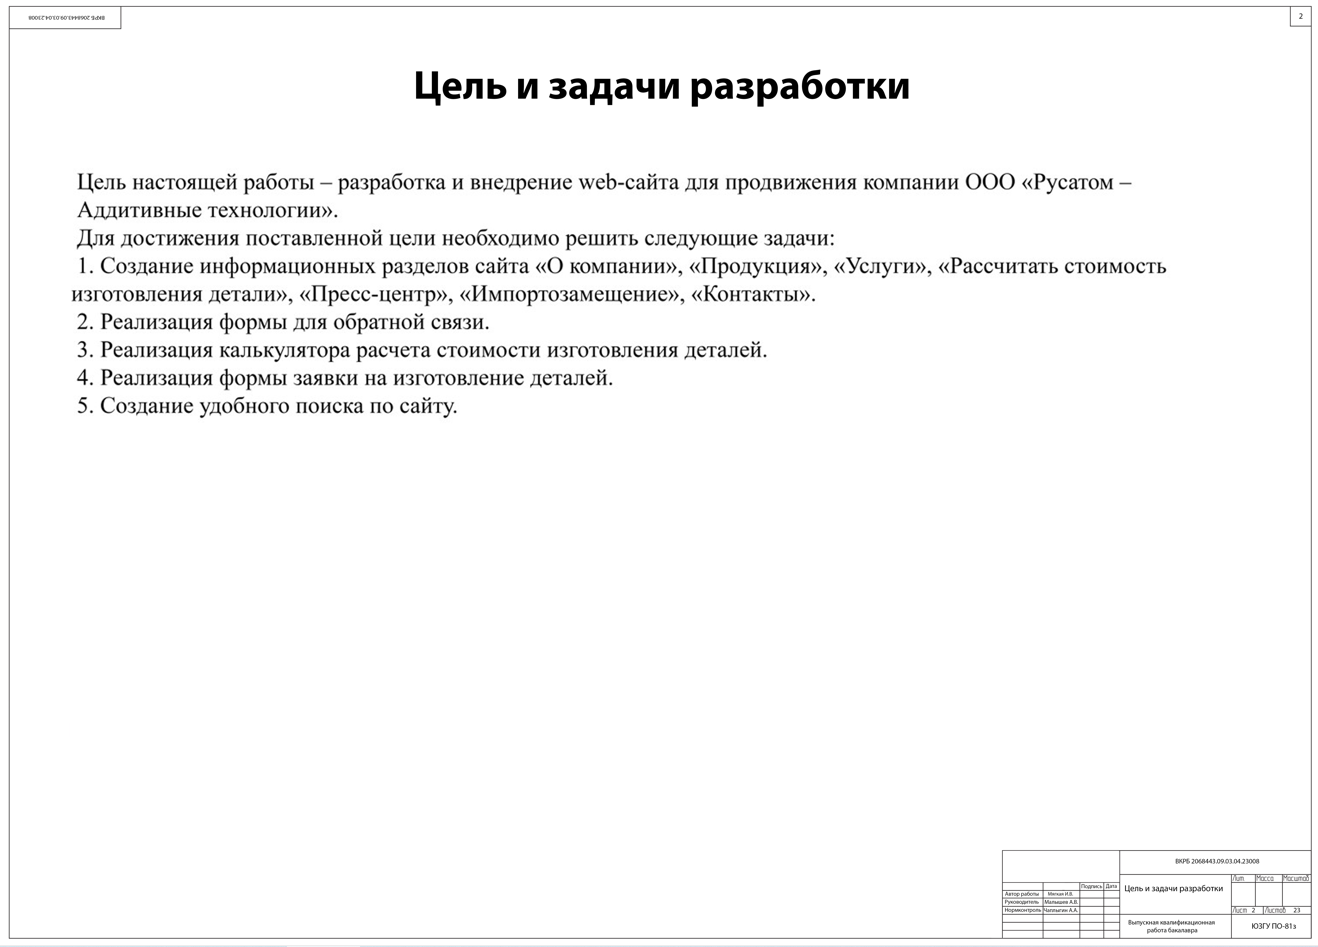
\includegraphics[width=0.82\linewidth]{плакат2.png}
    \заголовок{Цель и задачи разработки}
    \label{pl2:image}      
\end{плакат}

\begin{плакат}
    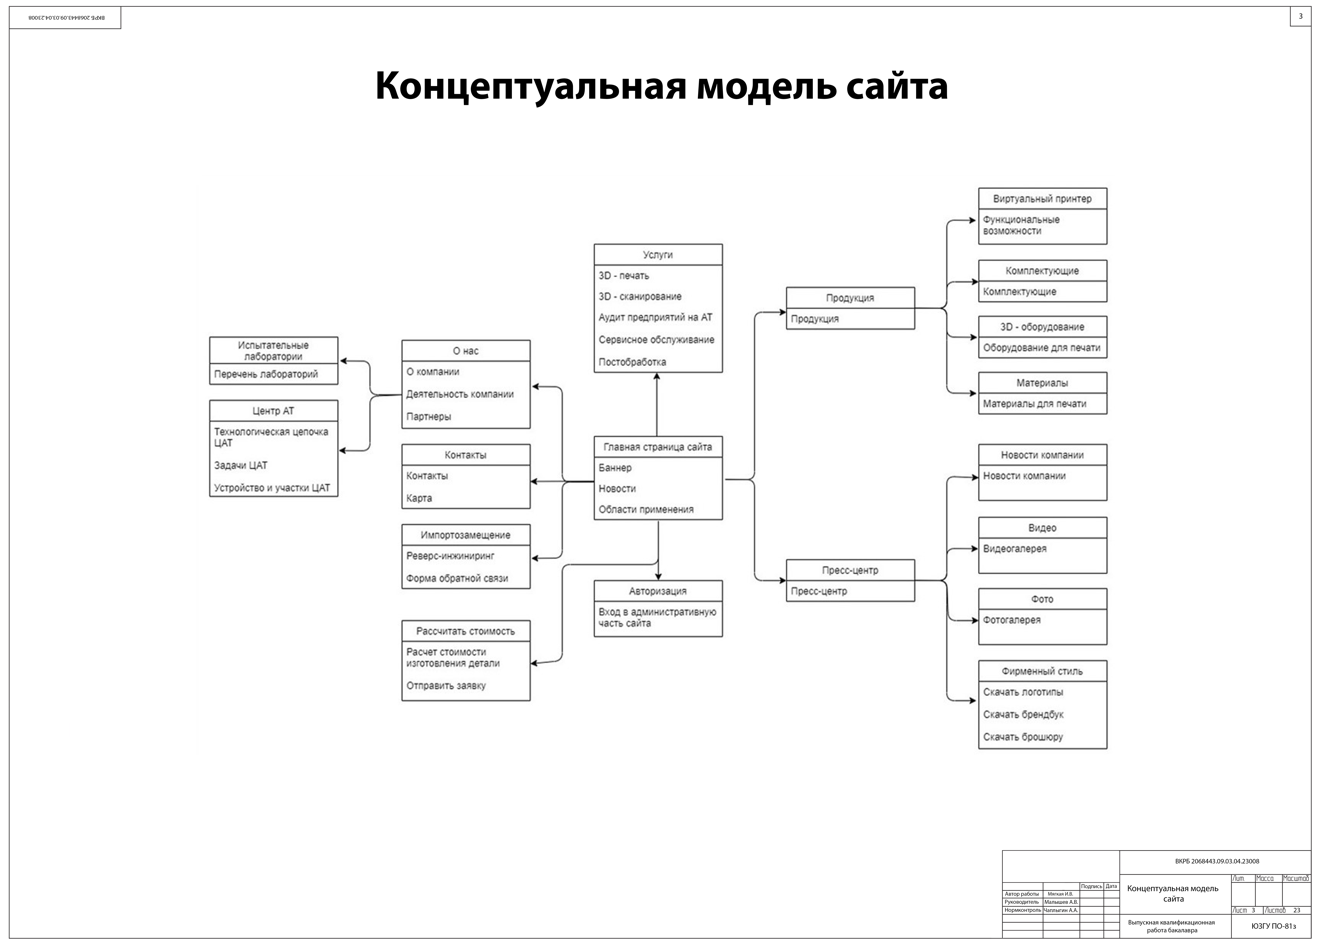
\includegraphics[width=0.82\linewidth]{плакат3.png}
    \заголовок{Концептуальная модель сайта}
    \label{pl3:image}      
\end{плакат}

\begin{плакат}
    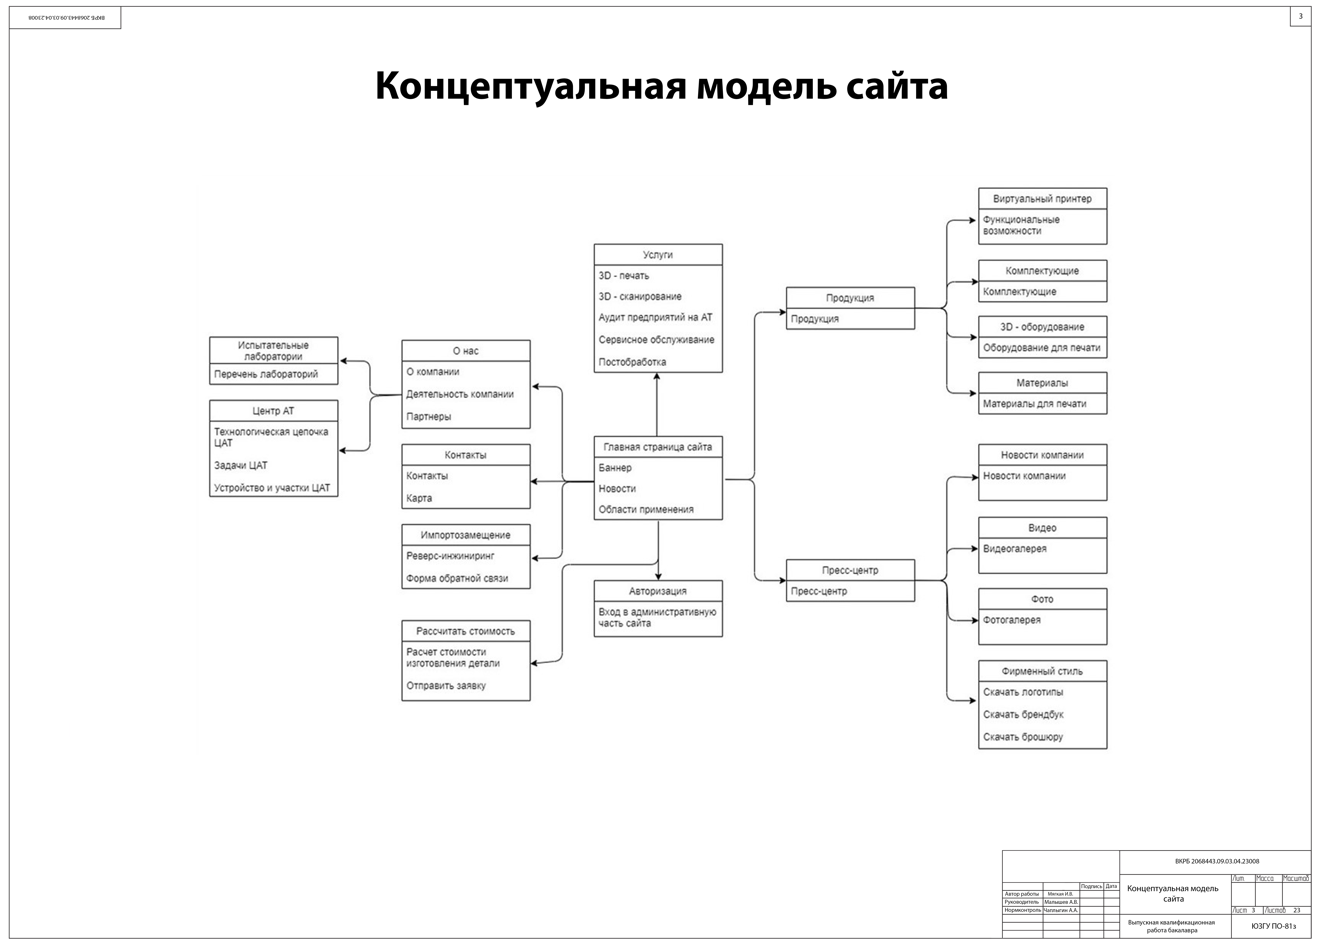
\includegraphics[width=0.82\linewidth]{плакат3.png}
    \заголовок{Еще плакат}
    \label{pl4:image}      
\end{плакат}

\end{landscape}
}\fi
\ifПрактика{}\else{\appendix{Фрагменты исходного кода программы}

main.py
\lstinputlisting[language=Python, frame=none]{main.py}

classifier.py
\lstinputlisting[language=Python, frame=none]{classifier.py}

training.py
\lstinputlisting[language=Python, frame=none]{training.py}

\ifВКР{
\newpage
\addcontentsline{toc}{section}{На отдельных листах (CD-RW в прикрепленном конверте)}
\begin{center}
\textbf{Место для диска}
\end{center}
}\fi
}\fi
\end{document}
